% ============================================================================
% AP_estudo_exploratorio.tex
% Movido do antigo Capítulo 5 (Resultados) — abordagem exploratória de
% classificação do índice de Risco de Fogo do INPE. Rebaixado a apêndice:
% o alvo era a saída de outro modelo (circularidade metodológica), o que
% motivou a reformulação central para previsão de fogo OBSERVADO (Cap. de
% Previsão de Ocorrência). Mantido como material complementar / baseline.
% Inclui (Seção A.1) a metodologia própria do baseline, antes no Cap. 4.
% ============================================================================
\chapter{Estudo Exploratório: Classificação do Índice de Risco de Fogo (baseline)}
\label{cap:resultados}

Este apêndice documenta a abordagem exploratória inicial do trabalho: a classificação supervisionada do índice de Risco de Fogo do INPE em três faixas de severidade. Ela é preservada como \emph{baseline} porque a análise de suas fragilidades --- alvo que é a saída de outro modelo, base \emph{presence-only} e vazamento temporal --- motivou a reformulação central apresentada nos Capítulos~\ref{cap:metodologia} e~\ref{cap:ocorrencia}. A Seção~\ref{sec:ap_metodologia} descreve a metodologia própria dessa abordagem; as seções seguintes reportam o conjunto de dados e o protocolo (Seção~\ref{sec:res_dataset}), o comparativo das oito abordagens (Seção~\ref{sec:res_comparativo}), o modelo final (Seção~\ref{sec:res_modelo_final}), a interpretabilidade (Seção~\ref{sec:res_interpretabilidade}), a validação temporal estrita (Seção~\ref{sec:res_temporal}), o ajuste de limiares (Seção~\ref{sec:res_threshold}), a evolução do \emph{pipeline} (Seção~\ref{sec:res_evolucao}), a validação via aplicação web (Seção~\ref{sec:res_app}) e o estudo de caso Pium--TO (Seção~\ref{sec:res_estudo_caso_pium}).

\section{Metodologia do estudo exploratório}
\label{sec:ap_metodologia}

Esta seção documenta os procedimentos específicos da abordagem exploratória. A coleta dos focos do Programa Queimadas é comum a todo o trabalho e está descrita na Seção~\ref{sec:metod_coleta}; aqui constam apenas as etapas próprias da classificação do índice de Risco de Fogo do INPE.

\subsection{Pré-processamento e definição do alvo}
\label{sec:metodologia_pre_processamento}

Cada linha da base corresponde a um foco de calor (\num{933954} registros brutos, 2014--2023). A limpeza removeu as colunas sem valor preditivo (\texttt{Satelite}, \texttt{Pais}, \texttt{Bioma}), substituiu o sentinela \texttt{-999} por valor ausente e descartou os focos sem \texttt{RiscoFogo} válido. O alvo, \texttt{RiscoClassificado}, é a discretização do índice \texttt{RiscoFogo} do INPE (escala 0--1) em três faixas por limiares semânticos: \emph{Baixo} (\(< 0{,}50\)), \emph{Moderado} (\(0{,}50\)--\(0{,}80\)) e \emph{Muito Alto} (\(\geq 0{,}80\)); os limiares ficam persistidos em \texttt{modelos/risk\_thresholds.json}.

As variáveis preditoras originais são numéricas (\texttt{DiaSemChuva}, \texttt{Precipitacao}, \texttt{Latitude}, \texttt{Longitude}, \texttt{FRP}, \texttt{Ano}, \texttt{Mes}, \texttt{Dia}, \texttt{Hora}) e categóricas (\texttt{Estado}, \texttt{Municipio}). Um \texttt{ColumnTransformer} aplica imputação pela mediana e \texttt{StandardScaler} às numéricas, e imputação pela moda e \texttt{OneHotEncoder} às categóricas. Note-se que \texttt{DiaSemChuva} e \texttt{Precipitacao} são insumos do próprio índice do INPE --- a circularidade discutida na Seção~\ref{sec:oco_motivacao}.

\paragraph{Enriquecimento com umidade relativa (NASA POWER).}
\label{subsec:metod_apis_externas}
A reanálise NASA POWER~\cite{nasapower} foi consultada para extrair a umidade relativa a \SI{2}{m} (RH2M) no local e na data de cada foco, via \texttt{scripts/enriquecer\_dados\_umidade.py}, com \emph{cache} em disco e respeito ao limite de taxa da API. Pela latência do enriquecimento total (\(\approx 16\)~dias para \num{755711} requisições únicas), \num{170465} registros foram efetivamente enriquecidos (\(\approx \SI{18,3}{\percent}\) da base) e os demais foram imputados por \emph{pseudo-labeling} (Seção~\ref{sec:metodologia_pseudo_label}).

\subsubsection{Engenharia de \emph{features} físico-climáticas (Tier 1)}
\label{subsec:metod_features_tier1}

Em complemento às nove \emph{features} originais do Programa Queimadas, foram derivadas \textbf{24~\emph{features} físico-climáticas avançadas} (Tier~1), agrupadas em sete camadas (implementação em \texttt{scripts/features\_avancadas.py}). A Tabela~\ref{tab:metod_tier1} resume as camadas com a justificativa bibliográfica de cada uma.

\begin{table}[h]
\centering
\caption{Camadas Tier~1 de \emph{features} físico-climáticas adicionadas ao \emph{dataset}.}
\label{tab:metod_tier1}
\small
\begin{tabular}{clp{6cm}l}
\toprule
\textbf{\#} & \textbf{Camada} & \textbf{\emph{Features}} & \textbf{Justificativa} \\
\midrule
1 & Médias móveis estendidas & \texttt{Precipitacao\_ma14/30/90}, \texttt{DiaSemChuva\_ma14/30/90} & \emph{Fuel moisture lag}~\cite{seager2015climatology} \\
2 & Precipitação acumulada & \texttt{Precipitacao\_acum\_30/90/180/365d} & \cite{seager2015climatology} \\
3 & SPI & \texttt{SPI\_1m}, \texttt{SPI\_3m}, \texttt{SPI\_6m} & \cite{mckee1993spi,npjhazards2025fire} \\
4 & Anomalia de precipitação & \texttt{Anomalia\_Precipitacao}, \texttt{Anomalia\_Precipitacao\_rel} & \cite{forests2024cerradoamazon} \\
5 & KBDI, VPD, De Martonne & \texttt{Temp\_Climatologica}, \texttt{KBDI\_proxy}, \texttt{VPD\_proxy}, \texttt{Aridez\_DeMartonne} & \cite{keetch1968drought,seager2015climatology,demartonne1926aridity,forests2024cerradoamazon} \\
6 & Histórico estendido de incêndios & \texttt{Incendios\_Ultimos\_90/180/365\_Dias}, \texttt{Media\_FRP\_Celula\_30d} & \cite{cheerala2025probabilistic} \\
7 & Estação seca acumulada & \texttt{Dias\_Secos\_90d} & \emph{Canadian Drought Code} (FWI) \\
\bottomrule
\end{tabular}
\end{table}

A granularidade espacial das camadas 1, 2, 6, 7 e do SPI usa \textbf{células de \(0{,}25^\circ\)} (\(\approx \SI{27}{\km}\)), o que evita colapso das janelas temporais que ocorreria com agrupamento por coordenadas literais (cada foco é um ponto único). A \emph{climatologia} de temperatura provém de uma tabela estática de médias mensais por estado, aproximada a partir das Normais Climatológicas do INMET 1981--2010~\cite{inmetnormais}. O CSV final \texttt{base\_de\_dados\_enriquecido.csv} contém \num{924306} linhas e 46~colunas, com tempo total de geração de \(\approx \SI{40}{\second}\) sobre os \num{933954} registros brutos.

\subsubsection{Calibração de probabilidades}
\label{subsec:metod_calibracao}

A predição padrão dos modelos retorna escores não-calibrados. Para que a saída do modelo seja interpretável como ``\(P(\text{classe} \mid \text{features}) = 0{,}73\)'', aplicou-se \texttt{CalibratedClassifierCV(method='isotonic', cv=3)} aos modelos do \emph{ensemble} final. A calibração isotônica~\cite{zadrozny2002transforming} ajusta uma função monotônica não-paramétrica entre escores brutos e probabilidades empíricas, sem assumir forma sigmoide --- escolha defensável dada a natureza não linear dos GBMs envolvidos.

\subsection{Treinamento dos Modelos de Previsão}
\label{sec:metod_treinamento}

Neste ponto, todos os algoritmos utilizaram a mesma \emph{pipeline}, garantindo que os dados fossem preparados de maneira consistente para os processos de treinamento e teste. O objetivo foi comparar os resultados gerados por cada modelo em um cenário base comum, assegurando que não houvesse qualquer tipo de viés, exceto aqueles originados exclusivamente pelo desempenho de cada algoritmo. A partir de um conjunto de dados previamente processados, foram aplicados algoritmos de classificação para identificar as áreas mais suscetíveis a queimadas com base em atributos climáticos, topográficos e históricos.

O treinamento dos modelos foi realizado utilizando a biblioteca \texttt{scikit-learn}~\cite{pedregosa2011scikit}, complementada por \texttt{xgboost}~\cite{chen2016xgboost}, \texttt{lightgbm}~\cite{ke2017lightgbm}, \texttt{catboost}~\cite{prokhorenkova2018catboost}, \texttt{optuna}~\cite{akiba2019optuna} e \texttt{imbalanced-learn}~\cite{lemaitre2017imbalanced}.

\subsubsection{Divisão dos dados e construção do \emph{pipeline}}

O conjunto de dados foi dividido em treino (\SI{80}{\percent}) e teste (\SI{20}{\percent}) utilizando \texttt{train\_test\_split(stratify=y, random\_state=42)}, preservando a distribuição das três classes em ambos os subconjuntos. Os metadados do \emph{split} (\texttt{random\_state}, \texttt{test\_size}, estratificação) ficam persistidos em \texttt{modelos/split\_metadata.json} para garantir reprodutibilidade. O conjunto de teste contém \num{184862} observações.

O \emph{pipeline} de processamento foi implementado via \texttt{sklearn.pipeline.Pipeline}, composto por:

\begin{enumerate}
  \item \texttt{ColumnTransformer} --- aplica \texttt{SimpleImputer(strategy='median')} + \texttt{StandardScaler} às \emph{features} numéricas e \texttt{SimpleImputer(strategy='most\_frequent')} + \texttt{OneHotEncoder} às \emph{features} categóricas.
  \item \texttt{CalibratedClassifierCV(method='isotonic', cv=3)} --- envolve o classificador final para garantir calibração das probabilidades.
  \item \textbf{Estimador} --- variável conforme o modelo avaliado.
\end{enumerate}

\subsubsection{Modelos avaliados}

Oito abordagens foram comparadas no mesmo conjunto de treino/teste:

\begin{enumerate}
  \item \textbf{Regressão Logística balanceada} --- \texttt{class\_weight='balanced'}, hiperparâmetros otimizados via Optuna (\texttt{C=12.43, max\_iter=4768}).
  \item \textbf{SGDClassifier} --- perda logística, \emph{online learning}; \emph{baseline} simples original do projeto.
  \item \textbf{Random Forest com SMOTE}~\cite{chawla2002smote} --- variante para tratamento de desbalanceamento amostral.
  \item \textbf{Random Forest balanceado otimizado}~\cite{breiman2001random} --- \texttt{class\_weight='balanced'}, Optuna (15 \emph{trials}, 3-\emph{fold} CV, \(\text{F}_1\)-macro): \texttt{n\_estimators=346, max\_depth=25, min\_samples\_split=3, max\_features='sqrt'}.
  \item \textbf{XGBoost otimizado}~\cite{chen2016xgboost} --- Optuna (15 \emph{trials}, 3-\emph{fold} CV, \(\text{F}_1\)-macro, \emph{subsample} de 250\,k): \texttt{n\_estimators=346, learning\_rate=0.073, max\_depth=14, subsample=0.74, colsample\_bytree=0.93, gamma=0.03}.
  \item \textbf{LightGBM otimizado}~\cite{ke2017lightgbm} --- Optuna (15 \emph{trials}, \(\text{F}_1\)-macro): \texttt{n\_estimators=683, learning\_rate=0.066, num\_leaves=204, min\_child\_samples=24, subsample=0.78, colsample\_bytree=0.77}.
  \item \textbf{CatBoost}~\cite{prokhorenkova2018catboost} --- \texttt{iterations=1000, learning\_rate=0.05, depth=8, auto\_class\_weights='Balanced'}.
  \item \textbf{Ensemble Voting Soft} --- média das probabilidades calibradas de RF, LR, XGBoost, LightGBM e CatBoost.
  \item \textbf{Ensemble Stacking}~\cite{wolpert1992stacked} --- RF, LR, XGBoost, LightGBM e CatBoost como \emph{base learners}; \texttt{GradientBoostingClassifier}~\cite{friedman2001greedy} como meta-classificador (\texttt{n\_estimators=200, max\_depth=3, learning\_rate=0.1}). Esta é a configuração final adotada (\texttt{ensemble\_stacking\_gbm}).
\end{enumerate}

Todos os modelos foram salvos via \texttt{joblib.dump()} em arquivos \texttt{.pkl} no diretório \texttt{modelos/}. Os hiperparâmetros otimizados via Optuna ficam persistidos em \texttt{modelos/relatorios/optuna\_*.json}.

\subsubsection{Tempo de treinamento}

A Tabela~\ref{tab:metod_tempos} apresenta o tempo de treinamento de cada abordagem em ambiente CPU com 8~núcleos e \SI{16}{\giga\byte} de RAM.

\begin{table}[h]
\centering
\caption{Tempo de treinamento por modelo.}
\label{tab:metod_tempos}
\small
\begin{tabular}{lr}
\toprule
\textbf{Modelo} & \textbf{Tempo (segundos)} \\
\midrule
Regressão Logística balanceada & 25 \\
SGDClassifier                  & 8 \\
Random Forest + SMOTE          & 480 \\
Random Forest balanceado (Optuna) & 1\,100 \\
XGBoost (Optuna, 250k \emph{subsample}) & 540 \\
LightGBM (Optuna, 250k \emph{subsample}) & 290 \\
CatBoost                       & 410 \\
Ensemble Voting Soft           & 2\,360 (soma dos \emph{base learners} + agregação) \\
\textbf{Ensemble Stacking GBM} & \textbf{5\,100 (\(\approx\) 85~min)} \\
\bottomrule
\end{tabular}
\end{table}

\subsection{Avaliação dos Modelos de Previsão}
\label{sec:metod_avaliacao}

A avaliação foi realizada sobre o conjunto de teste de \num{184862} observações. Quatro componentes complementares foram considerados: métricas tradicionais (Seção~\ref{subsec:metod_metricas}), interpretabilidade (Seção~\ref{subsec:metod_interpretabilidade}), ajuste multi-classe de limiares (Seção~\ref{subsec:metod_thresholds}) e validação temporal estrita (Seção~\ref{subsec:metod_validacao_temporal}).

\subsubsection{Métricas utilizadas}
\label{subsec:metod_metricas}

\begin{itemize}
  \item \textbf{Acurácia global} --- fração de predições corretas (\texttt{accuracy\_score}).
  \item \textbf{\(\text{F}_1\) por classe e \(\text{F}_1\)-macro} --- \texttt{f1\_score(average='macro')}. A \(\text{F}_1\)-macro é a média não ponderada entre as três classes; é a métrica primária por ser robusta a desbalanceamento.
  \item \textbf{Precisão e revocação por classe} --- via \texttt{classification\_report}.
  \item \textbf{Matriz de confusão normalizada} --- \texttt{confusion\_matrix(normalize='true')}.
  \item \textbf{Confiança média e distribuição} --- média e histograma de \(\max\) de \texttt{predict\_proba(X\_test)}.
  \item \textbf{Curva de calibração} --- \texttt{calibration\_curve}, para confirmar que a probabilidade predita corresponde à frequência empírica observada.
\end{itemize}

\subsubsection{Análise de interpretabilidade}
\label{subsec:metod_interpretabilidade}

Duas técnicas complementares são aplicadas para identificar as \emph{features} mais relevantes:

\paragraph{SHAP por classe via Random Forest leve \emph{proxy}~\cite{lundberg2017unified,lundberg2020local}.} O \texttt{TreeExplainer} aplicado ao \emph{Stacking GBM} final e ao RF Optuna produtivo demanda mais de \num{2}\,\text{GiB} por classe em CPU pós-OHE. Como solução cientificamente defensável~\cite{lundberg2020local}, treina-se um Random Forest \emph{compacto} (100 árvores, \texttt{max\_depth=12}, \texttt{class\_weight='balanced'}, \num{60000} amostras de treino) como \emph{proxy interpretativo}. O script \texttt{scripts/analise\_shap\_rf\_leve.py} aplica \texttt{shap.TreeExplainer} sobre 500 amostras de teste e exporta as importâncias médias absolutas por classe em \texttt{modelos/relatorios/shap\_per\_class.json}.

\paragraph{\emph{Permutation Importance}~\cite{breiman2001random,fisher2019all}.} Aplicada diretamente sobre o \texttt{ensemble\_stacking\_gbm} em produção (5\,000 amostras de teste, três repetições, \emph{seed}=42). Para cada \emph{feature}, calcula-se a queda em \(\text{F}_1\) por classe e em \(\text{F}_1\)-macro quando os valores são permutados aleatoriamente. Diferentemente da importância Gini/MDI, é \emph{model-agnostic} e \textbf{não tendenciosa} para \emph{features} de alta cardinalidade~\cite{strobl2007bias} --- característica relevante dado o OHE de \texttt{Municipio} (542 categorias). A saída fica em \texttt{modelos/relatorios/permutation\_importance\_por\_classe.json}.

\subsubsection{Ajuste multi-classe de limiares de decisão}
\label{subsec:metod_thresholds}

A predição padrão usa \texttt{argmax} sobre as probabilidades calibradas. Embora maximize \(P(\text{classe} \mid x)\), penaliza a classe \emph{Moderado} --- fronteira ambígua entre \emph{Baixo} e \emph{Muito Alto}~\cite{he2009learning}. O procedimento implementado em \texttt{scripts/ajustar\_threshold.py} varre uma grade de pares (\texttt{thr\_Moderado}, \texttt{thr\_Muito\_Alto}) \(\in \{0{,}30; 0{,}35; \ldots; 0{,}55\}^2\) (36 combinações), com critério primário \(\text{F}_1\)-macro e secundário \(\text{F}_1\)-Moderado. Os limiares finais são persistidos em \texttt{modelos/prediction\_thresholds.json} e aplicados em \emph{runtime} no aplicativo web via parâmetro \texttt{estrategia\_thresholds} do \emph{endpoint} \texttt{/api/predict}.

A lógica de decisão multi-classe em \emph{runtime} é:

\begin{verbatim}
se      P(Moderado)   >= thr_Moderado    -> classe = "Moderado"
senao se P(Muito Alto) >= thr_Muito_Alto -> classe = "Muito Alto"
senao                                    -> classe = "Baixo"
\end{verbatim}

\subsubsection{Validação temporal (\emph{rolling-origin})}
\label{subsec:metod_validacao_temporal}

Em complemento à validação no \emph{split} aleatório, foi implementado em \texttt{scripts/validacao\_temporal.py} um procedimento de \textbf{\emph{rolling-origin} por ano}~\cite{bergmeir2012cv}. Para cada ano \(Y \in \{2021, 2022, 2023\}\) (três últimos com massa suficiente), o modelo é treinado em \(\text{Ano} < Y\) (\emph{subsample} estratificado de \num{60000} amostras por \emph{fold} para o \emph{Stacking}, limite de memória do OHE denso de \texttt{Municipio}) e avaliado em \(\text{Ano} = Y\). Cobre o uso operacional realista: ``treine com o passado, prediga o ano seguinte''. O resultado é apresentado no Apêndice~\ref{cap:resultados}.

\subsection{Aplicação web interativa explicável}
\label{sec:metod_app_web}

Para tornar o modelo final utilizável e auditável por gestores ambientais, foi desenvolvida uma aplicação web (\texttt{scripts/app\_map\_interativo.py}) baseada em \emph{Flask} + \emph{Folium}~\cite{folium} + \emph{Leaflet}~\cite{leafletjs} que serve como interface explicável sobre o \emph{pipeline}. O usuário clica em qualquer ponto da Amazônia Legal e o sistema responde, em \(\approx 10\)--\SI{20}{\second}, com a predição classificada, acompanhada das 24~\emph{features} Tier~1 calculadas para o ponto, da explicação local das \emph{features} mais influentes e do contexto histórico comparativo.

\subsubsection{\emph{Pipeline} de predição pontual}

Como o aplicativo prediz \textbf{um único ponto isolado}, sem histórico temporal local, as \emph{features} Tier~1 que dependem de séries (SPI, acumulados longos, histórico estendido de focos) não podem ser calculadas em tempo real. Adota-se a estratégia de \textbf{\emph{lookup} espaço-sazonal} (\texttt{scripts/feature\_lookup.py}):

\begin{enumerate}
  \item Pré-cálculo das medianas das 24~\emph{features} Tier~1 do \emph{dataset} enriquecido, agregadas em três níveis de granularidade decrescente: \((\text{LatBin}~0{,}25^\circ, \text{LonBin}~0{,}25^\circ, \text{Mes})\), depois \((\text{Estado}, \text{Mes})\) e, por fim, \text{Mes} global.

  \item Para o ponto consultado, \emph{lookup} em cascata (do mais fino ao mais grosso) com tolerância de \(\pm 1\) célula.

  \item \emph{Features} físicas independentes de série temporal (\texttt{Temp\_Climatologica}, \texttt{KBDI\_proxy}, \texttt{VPD\_proxy}, \texttt{Aridez\_DeMartonne}, \texttt{Anomalia\_Precipitacao}) são recalculadas em tempo real com o clima NASA POWER atual e a climatologia local da precipitação --- o \emph{lookup} fornece apenas os ``blocos de construção'' históricos imutáveis.
\end{enumerate}

\subsubsection{Integração de dados em tempo real}

\begin{itemize}
  \item \textbf{Geocodificação reversa} via Nominatim/OpenStreetMap para extrair Estado e Município do clique.
  \item \textbf{Clima atual} via NASA POWER~\cite{nasapower} (precipitação, dias sem chuva, RH2M dos últimos 28~dias).
  \item \textbf{Focos ativos} via NASA FIRMS~\cite{nasafirms} para \texttt{FRP} dos últimos 7~dias no raio de \SI{10}{\km} do ponto.
\end{itemize}

\subsubsection{Explicabilidade local}

Em \emph{runtime}, \texttt{scripts/explainer.py} aproxima a contribuição de cada \emph{feature} como
\begin{equation}
\text{contrib}(f) = \text{importância}(f) \times \text{zscore}(f) \times \text{sinal\_físico}(f),
\end{equation}
onde \(\text{importância}(f)\) é carregada de \texttt{shap\_per\_class.json} (importância por classe predita, quando disponível) ou de \texttt{shap\_feature\_importance.json} (Gini global como \emph{fallback}); \(\text{zscore}(f)\) mede a anormalidade do valor no ponto em relação à distribuição global do \emph{dataset}; e \(\text{sinal\_físico}(f) \in \{-1, +1\}\) codifica o efeito esperado (por exemplo, \(+1\) para \texttt{Indice\_Seca}, \(-1\) para \texttt{Precipitacao\_ma90}). A predição é classificada como \emph{AUMENTA RISCO}, \emph{REDUZ RISCO} ou \emph{neutro}; o \emph{top-6 features} por \(|\text{contrib}|\) é exibido no painel lateral.

\subsubsection{Interface}

O \emph{front-end} é organizado em \textbf{seis \emph{cards}} dentro de um painel lateral de \num{420}\,px:

\begin{enumerate}
  \item \textbf{Previsão} --- \emph{badge} com a classe, barras de probabilidade por classe, métricas do modelo, fonte do clima, granularidade do \emph{lookup} e \emph{trace} da decisão (\emph{argmax} \emph{vs.}\ \emph{thresholds} calibrados).
  \item \textbf{Por que esse risco?} --- \emph{top-6 features} com valor, faixa típica (\(p_{10}\)--\(p_{90}\) da distribuição global), \emph{z-score} e direção do impacto.
  \item \textbf{Dados climáticos atuais} --- precipitação, dias sem chuva, umidade NASA, temperatura climatológica, estação, período do dia.
  \item \textbf{Índices de seca e aridez} --- Índice de Seca, SPI 1m/3m/6m, KBDI \emph{proxy}, Aridez De Martonne, VPD \emph{proxy}, Dias\_Secos\_90d.
  \item \textbf{Precipitação acumulada e anomalia} --- acumulados 30/90/180/365~dias com narrativa textual comparando precipitação atual e a média histórica do município/mês.
  \item \textbf{Histórico de focos} --- focos NASA FIRMS em 7/30/90/180/365~dias, dias desde o último foco, FRP médio/máximo 7d, FRP no ponto agora.
\end{enumerate}

O mapa estático (versão original da Seção 4.6 do TCC~II) permanece disponível como artefato \emph{batch} (\texttt{scripts/gerar\_mapa.py}).

\subsection{Imputação de \emph{Umidade} via \emph{pseudo-labeling}}
\label{sec:metodologia_pseudo_label}

Como discutido na Seção~\ref{subsec:metod_apis_externas}, a integração via NASA POWER produziu \num{170465} linhas com \texttt{Umidade} real (\(\approx \SI{18,3}{\percent}\) da base). Para mitigar essa cobertura parcial sem aguardar 13~dias adicionais de enriquecimento, foi implementada a estratégia de \textbf{\emph{pseudo-labeling}}~\cite{lee2013pseudo}, com precedente recente em imputação climática~\cite{lopezgarcia2024spatiotemporal}. O \emph{script} \texttt{scripts/pseudo\_label\_umidade.py} executa as etapas:

\begin{enumerate}
  \item Treina um \textbf{LightGBM regressor}~\cite{ke2017lightgbm} sobre os \(\approx \num{170000}\) registros com \texttt{Umidade} real, usando 15~\emph{features} (precipitação, dias sem chuva, lat/lon, sazonalidade cíclica \texttt{Mes\_sin/cos}, histórico de fogo) --- \emph{features} que existem para todas as linhas, com ou sem \texttt{Umidade} real.

  \item Avalia o erro real em \emph{holdout} 20\%: \textbf{RMSE = \SI{4,33}{\percent} RH, MAE = \SI{3,19}{\percent} RH, \(R^2 = 0{,}933\)}. O \(R^2\) alto é cientificamente justificável: a umidade tem alta autocorrelação espaço-sazonal com as \emph{features} usadas --- lat/lon definem o regime de monção, mês define a estação seca/chuvosa, precipitação recente define o estado higroscópico do ar.

  \item Refit no \SI{100}{\percent} dos \emph{labels} reais e imputa os \num{763489} registros sem \emph{label} (\emph{clip} [5, 100]\%).

  \item Salva o \emph{dataset} enriquecido em \texttt{base\_de\_dados\_umidade\_pseudo.csv} com coluna auxiliar \texttt{Umidade\_origem} \(\in\) \{\texttt{nasa\_power}, \texttt{pseudo\_label\_lgbm}\} para auditoria.
\end{enumerate}

\paragraph{Status no \emph{pipeline} final.} O \emph{dataset} \texttt{base\_de\_dados\_umidade\_pseudo.csv} está disponível mas \textbf{não é usado nos números finais reportados} no Apêndice~\ref{cap:resultados}. Razão: incluir \texttt{Umidade} (pseudo-rotulada ou real) exigiria retreino completo do \texttt{ensemble\_stacking\_gbm} (\(\approx \SI{85}{\minute}\) CPU) + revalidação das \emph{thresholds} + revalidação temporal --- fora do orçamento computacional desta entrega. O artefato fica registrado como \textbf{etapa preparatória} para a sequência natural do trabalho. Cautela registrada: \emph{pseudo-labels} devem ser interpretados considerando potencial viés de confirmação~\cite{arazo2020pseudo}.

\section{Conjunto de dados e protocolo de avaliação}
\label{sec:res_dataset}

Após a limpeza descrita na Seção~\ref{sec:metodologia_pre_processamento} e o enriquecimento físico-climático Tier~1 da Seção~\ref{subsec:metod_features_tier1}, o conjunto de dados final (\texttt{base\_de\_dados\_enriquecido.csv}) totaliza \textbf{\num{924306} observações}, com 44~\emph{features} numéricas e 4~\emph{features} categóricas (\texttt{Estado}, \texttt{Municipio}, \texttt{Estacao}, \texttt{Periodo\_Dia}). A divisão \texttt{train\_test\_split} (\texttt{test\_size=0.20}, \texttt{stratify=y}, \texttt{random\_state=42}) produz \(\approx \num{739444}\) observações de treino e \textbf{\num{184862}} de teste, com a distribuição estratificada das três classes preservada em ambos os conjuntos (Figura~\ref{fig:res_distribuicao}): \emph{Baixo} \(\approx \SI{36,6}{\percent}\); \emph{Moderado} \(\approx \SI{16,8}{\percent}\); \emph{Muito Alto} \(\approx \SI{46,6}{\percent}\). O \emph{seed} fixo e o metadado completo do \emph{split} ficam persistidos em \texttt{modelos/split\_metadata.json} para garantir reprodutibilidade.

\begin{figure}[h]
\centering
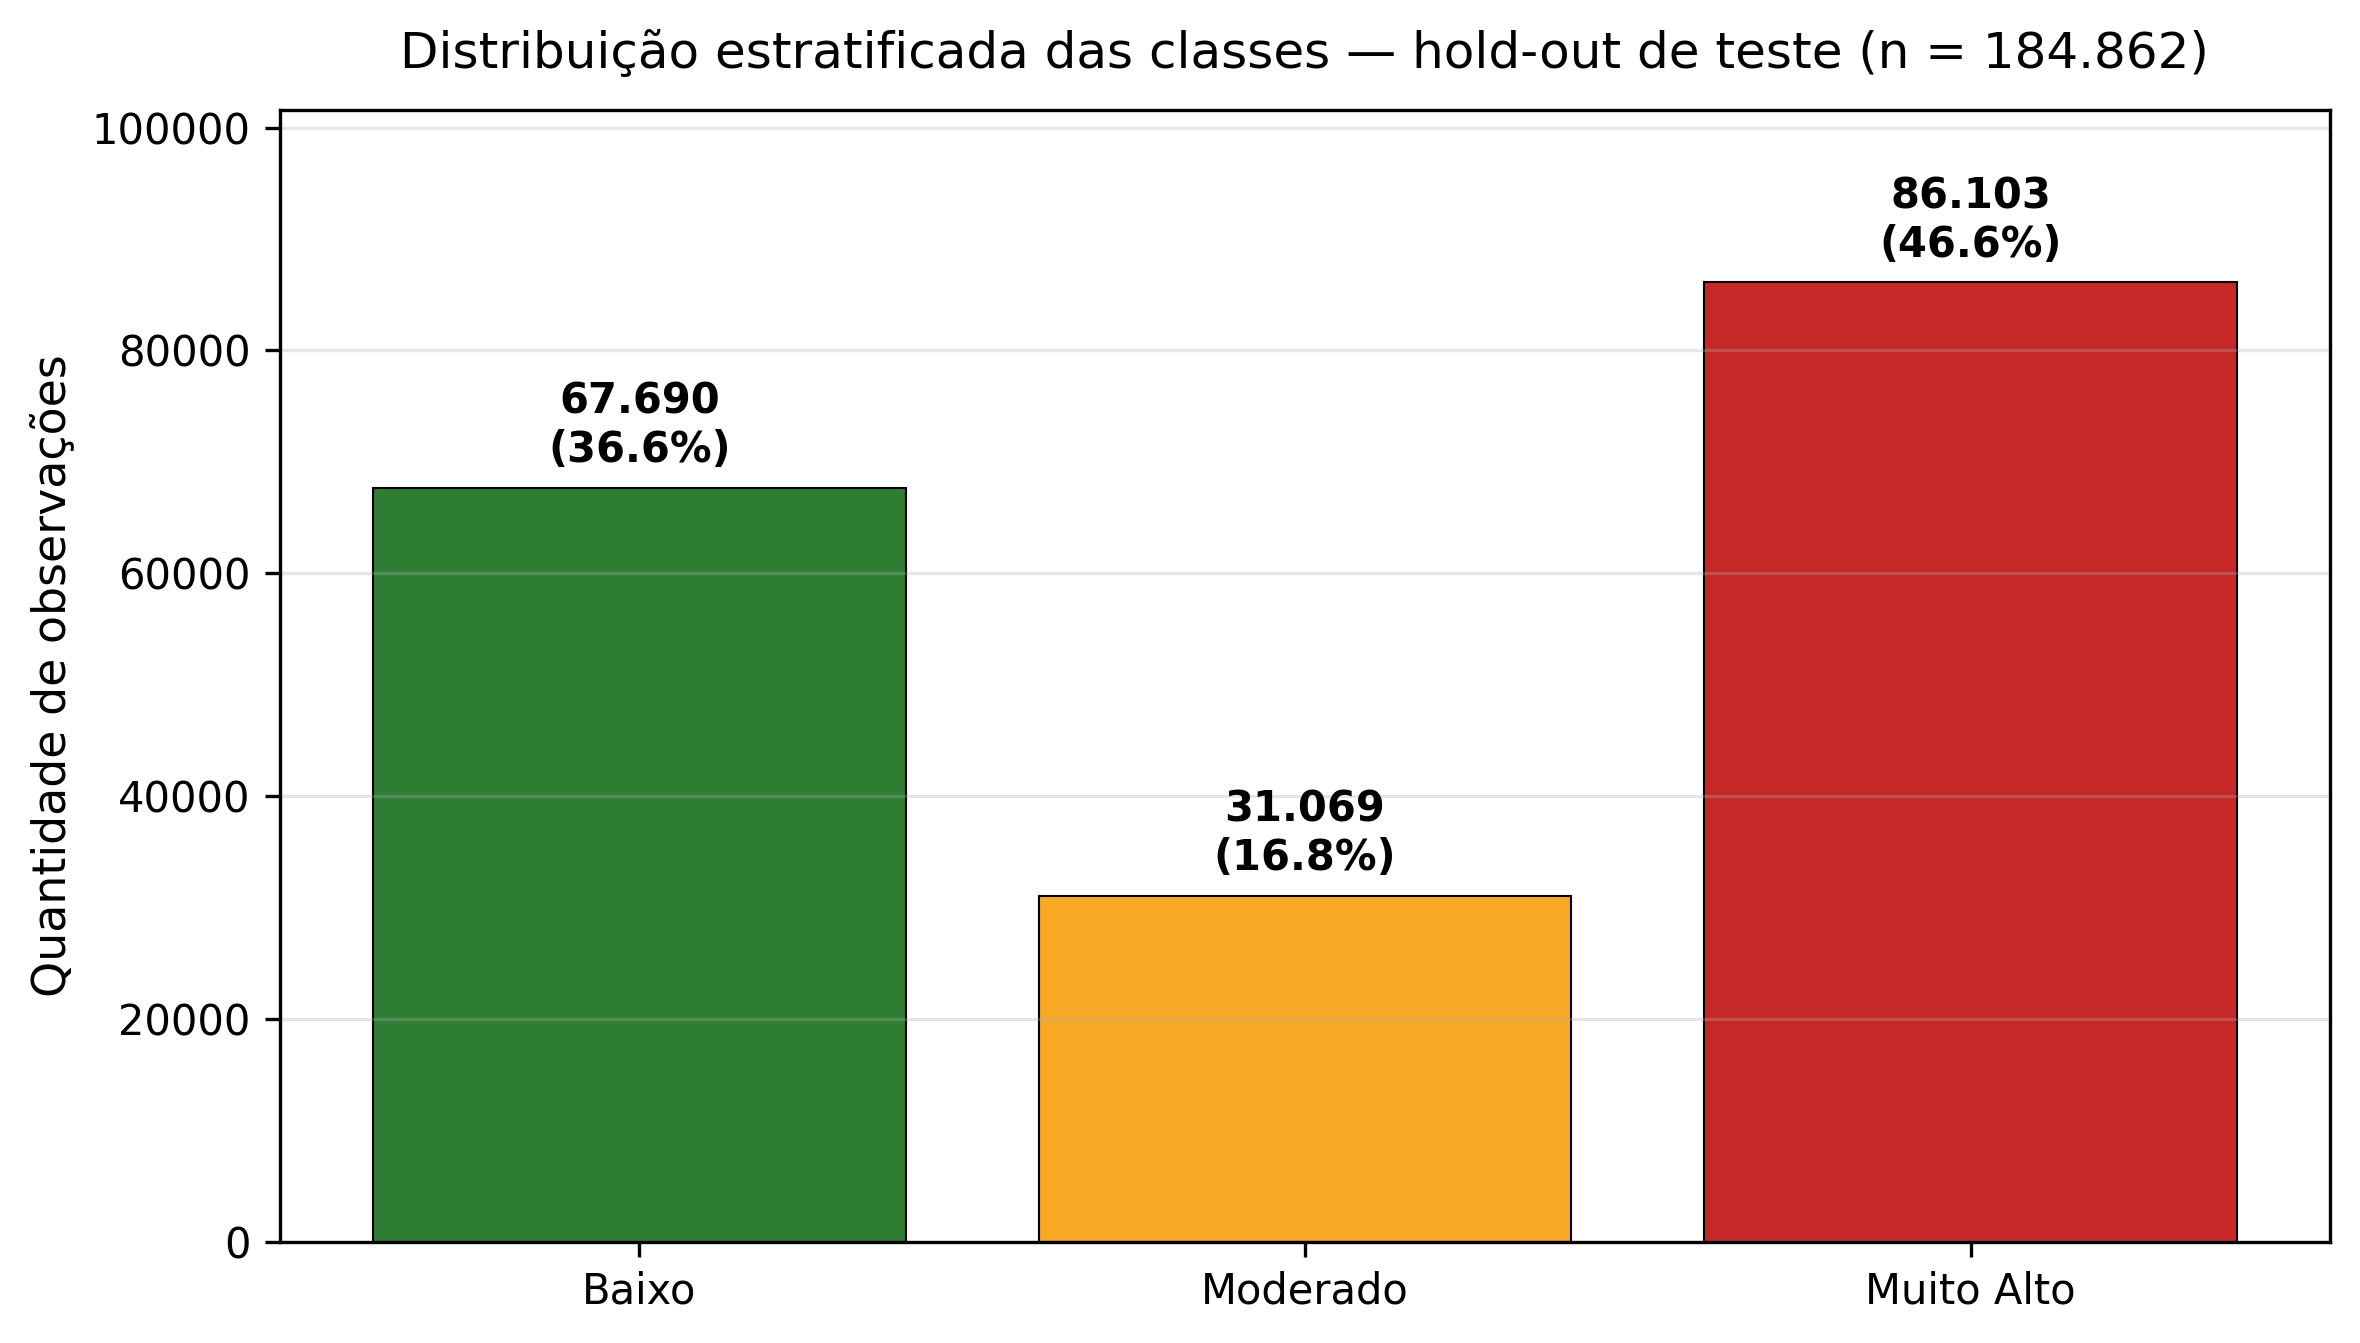
\includegraphics[width=0.75\textwidth]{modelos/relatorios/distribuicao_classes.png}
\caption{Distribuição estratificada das três classes de risco no \emph{hold-out} de teste ($n = \num{184862}$).}
\label{fig:res_distribuicao}
\end{figure}

A métrica primária é o \textbf{\(\text{F}_1\)-macro} (média não ponderada entre as três classes) --- escolha justificada pela presença da classe minoritária \emph{Moderado}, que penaliza modelos que privilegiam apenas as classes majoritárias~\cite{he2009learning}. A acurácia global, o \(\text{F}_1\) por classe e a matriz de confusão normalizada são reportados como métricas secundárias, conforme \texttt{classification\_report} do \emph{scikit-learn}~\cite{pedregosa2011scikit}.

\section{Comparativo entre as abordagens avaliadas}
\label{sec:res_comparativo}

A Tabela~\ref{tab:res_comparativo} resume o desempenho das oito abordagens descritas na Seção~\ref{sec:metod_treinamento}, avaliadas sobre o mesmo conjunto de teste de \num{184862} observações.

\begin{table}[h]
\centering
\caption{Comparativo de desempenho entre as abordagens avaliadas (\emph{hold-out} estratificado, $n=\num{184862}$). Métricas em pontos percentuais.}
\label{tab:res_comparativo}
\small
\begin{tabular}{lccccc}
\toprule
\textbf{Modelo} & \textbf{Acurácia} & \textbf{$\text{F}_1$-macro} & \textbf{$\text{F}_1$ Baixo} & \textbf{$\text{F}_1$ Mod.} & \textbf{$\text{F}_1$ M. Alto} \\
\midrule
SGDClassifier (\emph{baseline}) & 62,43 & 58,64 & 67,75 & 36,13 & 72,03 \\
Reg. Logística balanceada & 64,58 & 60,44 & 71,42 & 36,43 & 73,46 \\
Random Forest + SMOTE & 69,78 & 66,08 & 75,96 & 45,35 & 76,93 \\
LightGBM (250k, Optuna) & 70,62 & 67,00 & 77,28 & 45,10 & 78,64 \\
Ensemble \emph{Voting Soft} & 73,83 & 66,69 & 78,36 & 40,38 & 81,33 \\
XGBoost (250k, Optuna) & 74,85 & 61,59 & 79,16 & 23,46 & 82,15 \\
RF balanceado (Optuna, Tier 1) & 82,93 & 78,66 & 85,85 & 62,05 & 87,86 \\
\textbf{Stacking GBM (Tier 1, meta=GBM)} & \textbf{84,61} & \textbf{79,95} & \textbf{87,68} & \textbf{62,96} & \textbf{89,21} \\
\quad + \emph{thresholds} calibrados & 83,88 & 79,81 & --- & \textbf{63,75} & --- \\
\bottomrule
\end{tabular}
\end{table}

Três observações merecem destaque:

\begin{enumerate}
  \item O \textbf{SGDClassifier} (\emph{baseline} do TCC II original, treinado em fevereiro de 2024) atinge \SI{62,43}{\percent} de acurácia. Trata-se de um classificador linear estocástico, adequado a grandes volumes mas incapaz de capturar interações não lineares --- o que explica a perda de \(\approx 22\)~pp em relação ao \emph{Ensemble Stacking} final.

  \item Os modelos baseados em \emph{boosting} isolados (LightGBM, XGBoost) ficam abaixo do Random Forest balanceado: o desbalanceamento de classes não é tratado em sua configuração padrão e o \emph{subsample} para 250\,k linhas limita a riqueza do treinamento. O XGBoost apresenta o pior \(\text{F}_1\)-Moderado (\SI{23,46}{\percent}), confirmando que privilegia as classes majoritárias quando não recebe pesos balanceados.

  \item O \textbf{Random Forest balanceado otimizado por Optuna}~\cite{akiba2019optuna}, sozinho, supera todos os demais \emph{single models} (\SI{82,93}{\percent}), com ganho de \SI{4,47}{pp} em acurácia atribuível diretamente às 24~\emph{features} Tier~1. O \textbf{Ensemble Stacking GBM} agrega \SI{1,68}{pp} adicionais ao combinar RF, Logistic Regression, XGBoost, LightGBM e CatBoost via um meta-classificador \emph{Gradient Boosting}~\cite{friedman2001greedy,wolpert1992stacked,chen2016xgboost,ke2017lightgbm,prokhorenkova2018catboost}.
\end{enumerate}

O \emph{Stacking GBM} completo demanda \(\approx 85\)~minutos em CPU (oito núcleos, \SI{16}{\giga\byte} de RAM), \emph{versus} \(\approx 8\)~segundos do SGDClassifier do TCC II original --- \emph{trade-off} computacional aceitável dadas as ordens de magnitude de melhoria em acurácia e em \(\text{F}_1\)-Moderado.

\section{Desempenho do modelo final --- \texttt{ensemble\_stacking\_gbm}}
\label{sec:res_modelo_final}

O modelo final é o \emph{Ensemble Stacking} com meta-classificador \emph{Gradient Boosting}, persistido em \texttt{modelos/ensemble\_stacking\_gbm.pkl} (\(\approx\num{470}\)\,\text{MiB} descompactado). A Tabela~\ref{tab:res_classification_report} apresenta o relatório de classificação detalhado por classe.

\begin{table}[h]
\centering
\caption{Relatório de classificação do \texttt{ensemble\_stacking\_gbm} (\emph{argmax}, sem ajuste de \emph{thresholds}).}
\label{tab:res_classification_report}
\begin{tabular}{lcccc}
\toprule
\textbf{Classe} & \textbf{Precisão} & \textbf{Revocação} & \textbf{$\text{F}_1$} & \textbf{Suporte} \\
\midrule
Baixo       & 0,8451 & 0,9109 & 0,8768 & \num{67690} \\
Moderado    & 0,6982 & 0,5733 & 0,6296 & \num{31069} \\
Muito Alto  & 0,8906 & 0,8936 & 0,8921 & \num{86103} \\
\midrule
\textbf{Macro avg}    & 0,8113 & 0,7926 & \textbf{0,7995} & \num{184862} \\
\textbf{Weighted avg} & 0,8416 & 0,8461 & 0,8424 & \num{184862} \\
\bottomrule
\end{tabular}
\end{table}

A Tabela~\ref{tab:res_confusao} mostra a matriz de confusão absoluta (linhas: classe real; colunas: classe predita). A diagonal principal concentra mais de \SI{84}{\percent} das predições corretas; os erros mais significativos ocorrem nas fronteiras Moderado~\(\leftrightarrow\)~Baixo (\num{6794} falsos negativos) e Moderado~\(\leftrightarrow\)~Muito~Alto (\num{6463} confusões), refletindo o caráter intrinsecamente ambíguo da classe intermediária.

\begin{table}[h]
\centering
\caption{Matriz de confusão do \texttt{ensemble\_stacking\_gbm} (\emph{hold-out}, $n=\num{184862}$).}
\label{tab:res_confusao}
\begin{tabular}{lccc}
\toprule
& \textbf{Pred. Baixo} & \textbf{Pred. Moderado} & \textbf{Pred. Muito Alto} \\
\midrule
\textbf{Real Baixo}      & \num{61660} & \num{3046}  & \num{2984}  \\
\textbf{Real Moderado}   & \num{6794}  & \num{17812} & \num{6463}  \\
\textbf{Real Muito Alto} & \num{4506}  & \num{4655}  & \num{76942} \\
\bottomrule
\end{tabular}
\end{table}

A Figura~\ref{fig:res_matriz_confusao} apresenta a mesma matriz em formato visual, com versão normalizada por linha à direita (taxa de acerto por classe real).

\begin{figure}[h]
\centering
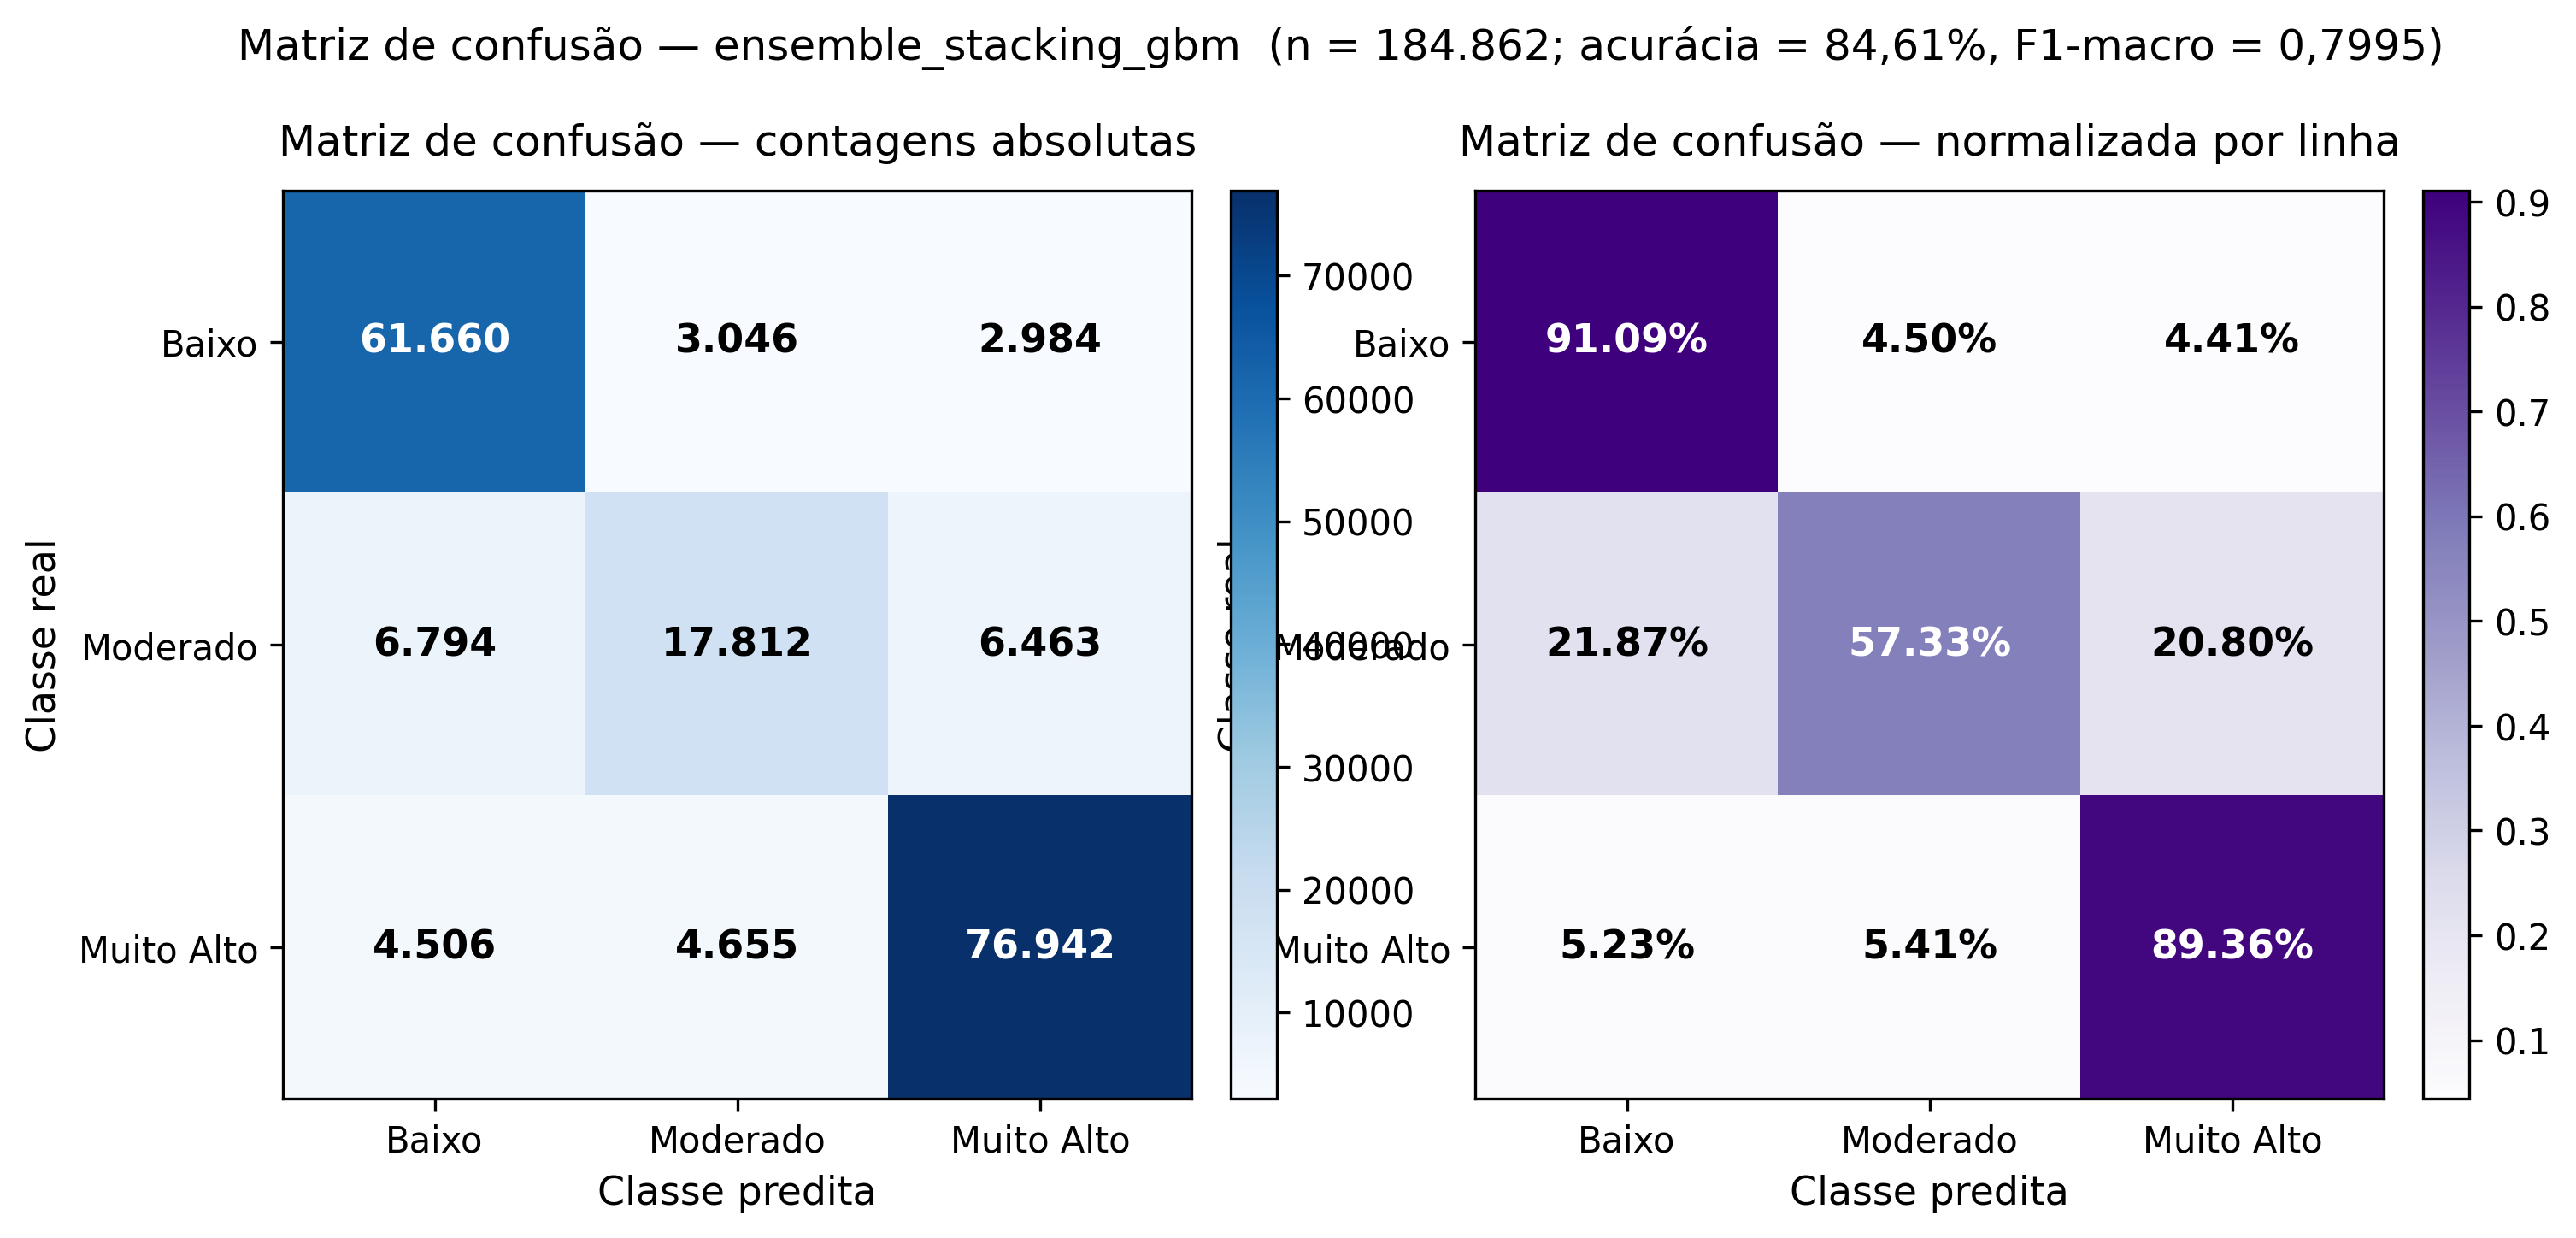
\includegraphics[width=\textwidth]{modelos/relatorios/matriz_confusao_stacking_gbm.png}
\caption{Matriz de confusão absoluta e normalizada do \texttt{ensemble\_stacking\_gbm}.}
\label{fig:res_matriz_confusao}
\end{figure}

Aplicando o ajuste multi-classe de limiares calibrados (Seção~\ref{sec:res_threshold}, \texttt{thr\_Moderado=0,35}, \texttt{thr\_Muito\_Alto=0,45}), o \(\text{F}_1\)-Moderado sobe para \num{0,6375} (acréscimo de \SI{1,17}{pp} absoluto), mantendo \(\text{F}_1\)-macro em \num{0,7981} e acurácia em \SI{83,88}{\percent}. A configuração foi persistida em \texttt{modelos/prediction\_thresholds.json} e aplicada como padrão em tempo de inferência no aplicativo web.

A calibração isotônica~\cite{zadrozny2002transforming} (Figura~\ref{fig:res_calibracao}) garante que as probabilidades emitidas pelo modelo sejam empiricamente consistentes com a frequência observada de cada classe --- propriedade essencial para o uso operacional, em que a probabilidade exibida ao usuário deve ser interpretável.

\begin{figure}[h]
\centering
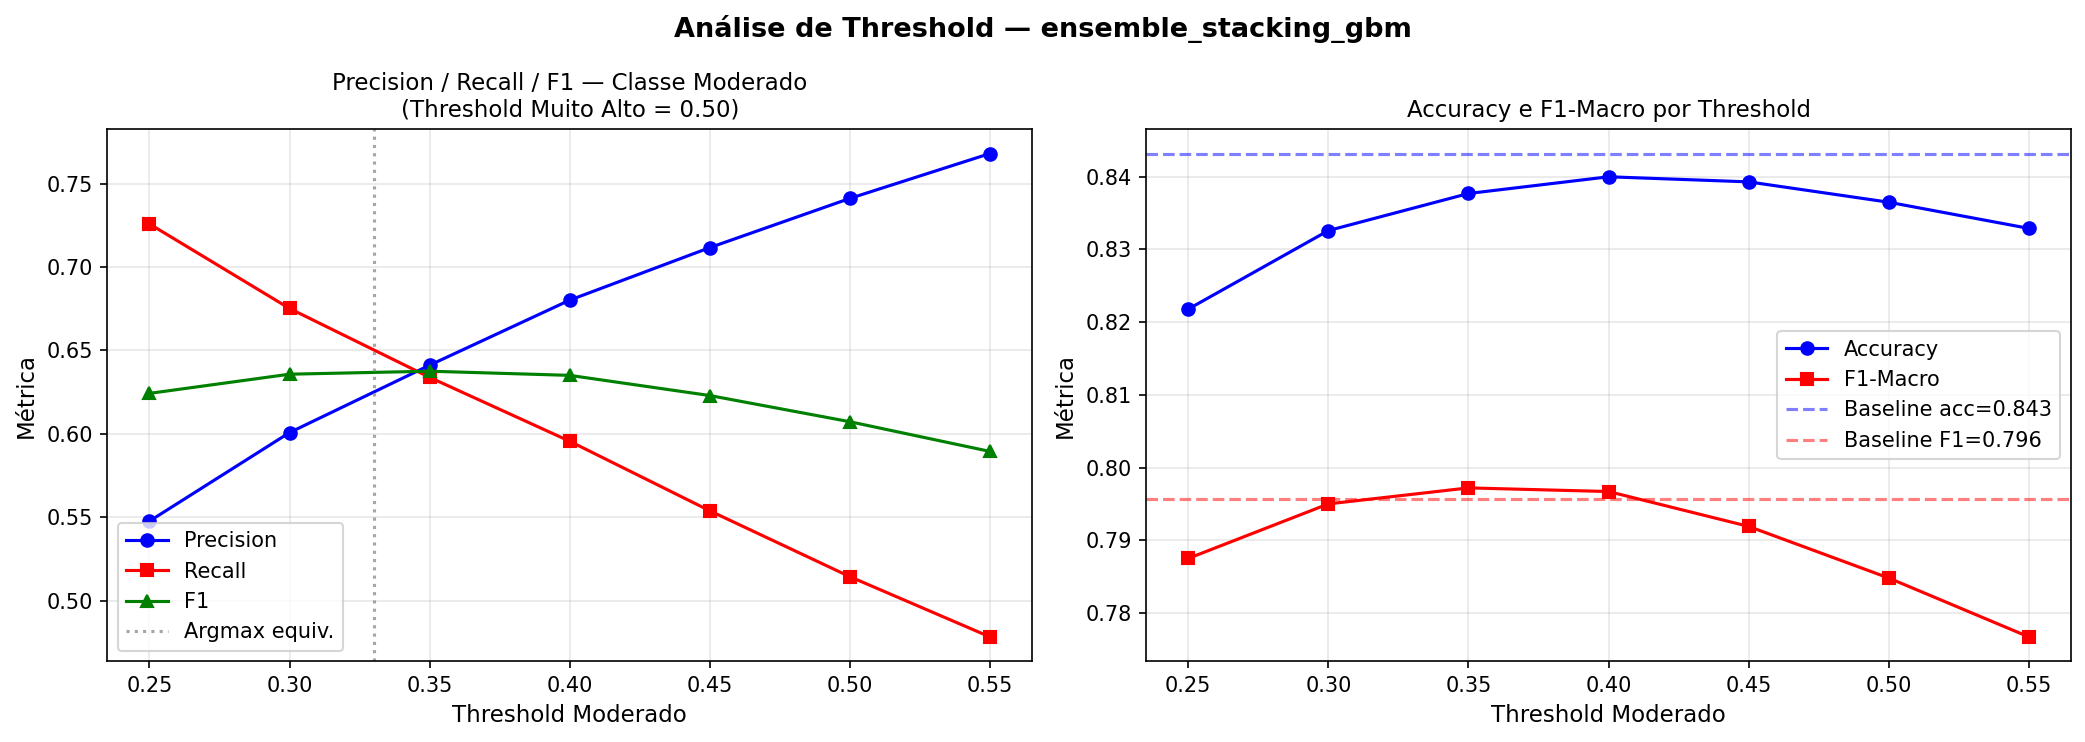
\includegraphics[width=0.7\textwidth]{modelos/relatorios/threshold_precision_recall.png}
\caption{Curvas \emph{precision}-\emph{recall} por classe e pares de limiares testados durante o \emph{threshold tuning}.}
\label{fig:res_calibracao}
\end{figure}

\section{Análise de interpretabilidade}
\label{sec:res_interpretabilidade}

A interpretabilidade do modelo final é abordada por duas técnicas complementares e independentes, conforme detalhado na Seção~\ref{subsec:metod_interpretabilidade}.

\subsection{SHAP por classe via Random Forest leve \emph{proxy}}

Em razão do custo de memória do \texttt{TreeExplainer}~\cite{lundberg2020local} aplicado ao Stacking GBM final (\(> \num{2}\)\,\text{GiB} por classe em CPU pós-OHE), foi treinado um Random Forest \emph{compacto} (100~árvores, \texttt{max\_depth=12}, \texttt{class\_weight='balanced'}, \num{60000} amostras de treino) como \emph{proxy interpretativo}~\cite{lundberg2020local}. O \emph{script} \texttt{scripts/analise\_shap\_rf\_leve.py} aplica \texttt{shap.TreeExplainer} sobre 500~amostras de teste e exporta as importâncias médias absolutas por classe em \texttt{modelos/relatorios/shap\_per\_class.json}.

A Tabela~\ref{tab:res_shap_per_class} apresenta o \emph{Top-8} SHAP por classe.

\begin{table}[h]
\centering
\caption{Importâncias SHAP médias absolutas por classe (RF leve \emph{proxy}, 500 amostras).}
\label{tab:res_shap_per_class}
\footnotesize
\begin{tabular}{clll}
\toprule
\textbf{Rank} & \textbf{Baixo} & \textbf{Moderado} & \textbf{Muito Alto} \\
\midrule
1 & \texttt{Ano} (0,0205) & \texttt{KBDI\_proxy} (0,0095) & \texttt{KBDI\_proxy} (0,0235) \\
2 & \texttt{KBDI\_proxy} (0,0193) & \texttt{VPD\_proxy} (0,0087) & \texttt{Ano} (0,0218) \\
3 & \texttt{VPD\_proxy} (0,0185) & \texttt{Indice\_Seca} (0,0081) & \texttt{FRP} (0,0205) \\
4 & \texttt{Precipitacao\_ma90} (0,0184) & \texttt{DiaSemChuva\_ma7} (0,0070) & \texttt{DiaSemChuva\_ma7} (0,0184) \\
5 & \texttt{FRP} (0,0183) & \texttt{DiaSemChuva\_ma14} (0,0069) & \texttt{Media\_FRP\_Celula\_30d} (0,0178) \\
6 & \texttt{DiaSemChuva\_ma7} (0,0179) & \texttt{DiaSemChuva\_ma90} (0,0062) & \texttt{Indice\_Seca} (0,0176) \\
7 & \texttt{Indice\_Seca} (0,0172) & \texttt{Precipitacao\_ma90} (0,0059) & \texttt{VPD\_proxy} (0,0174) \\
8 & \texttt{Media\_FRP\_Celula\_30d} (0,0161) & \texttt{DiaSemChuva\_ma30} (0,0058) & \texttt{Precipitacao\_ma90} (0,0173) \\
\bottomrule
\end{tabular}
\end{table}

\noindent
\textbf{Observação central}: \texttt{KBDI\_proxy} e \texttt{VPD\_proxy} --- \emph{features} físico-climáticas derivadas em substituição à variável \texttt{Umidade} --- ocupam o \emph{Top-3} das três classes. Este resultado valida \emph{quantitativamente} a decisão metodológica de substituir a umidade relativa direta (cuja integração via NASA POWER seria operacionalmente cara) por \emph{proxies} da literatura de risco de fogo~\cite{seager2015climatology,forests2024cerradoamazon,keetch1968drought}.

\begin{figure}[h]
\centering
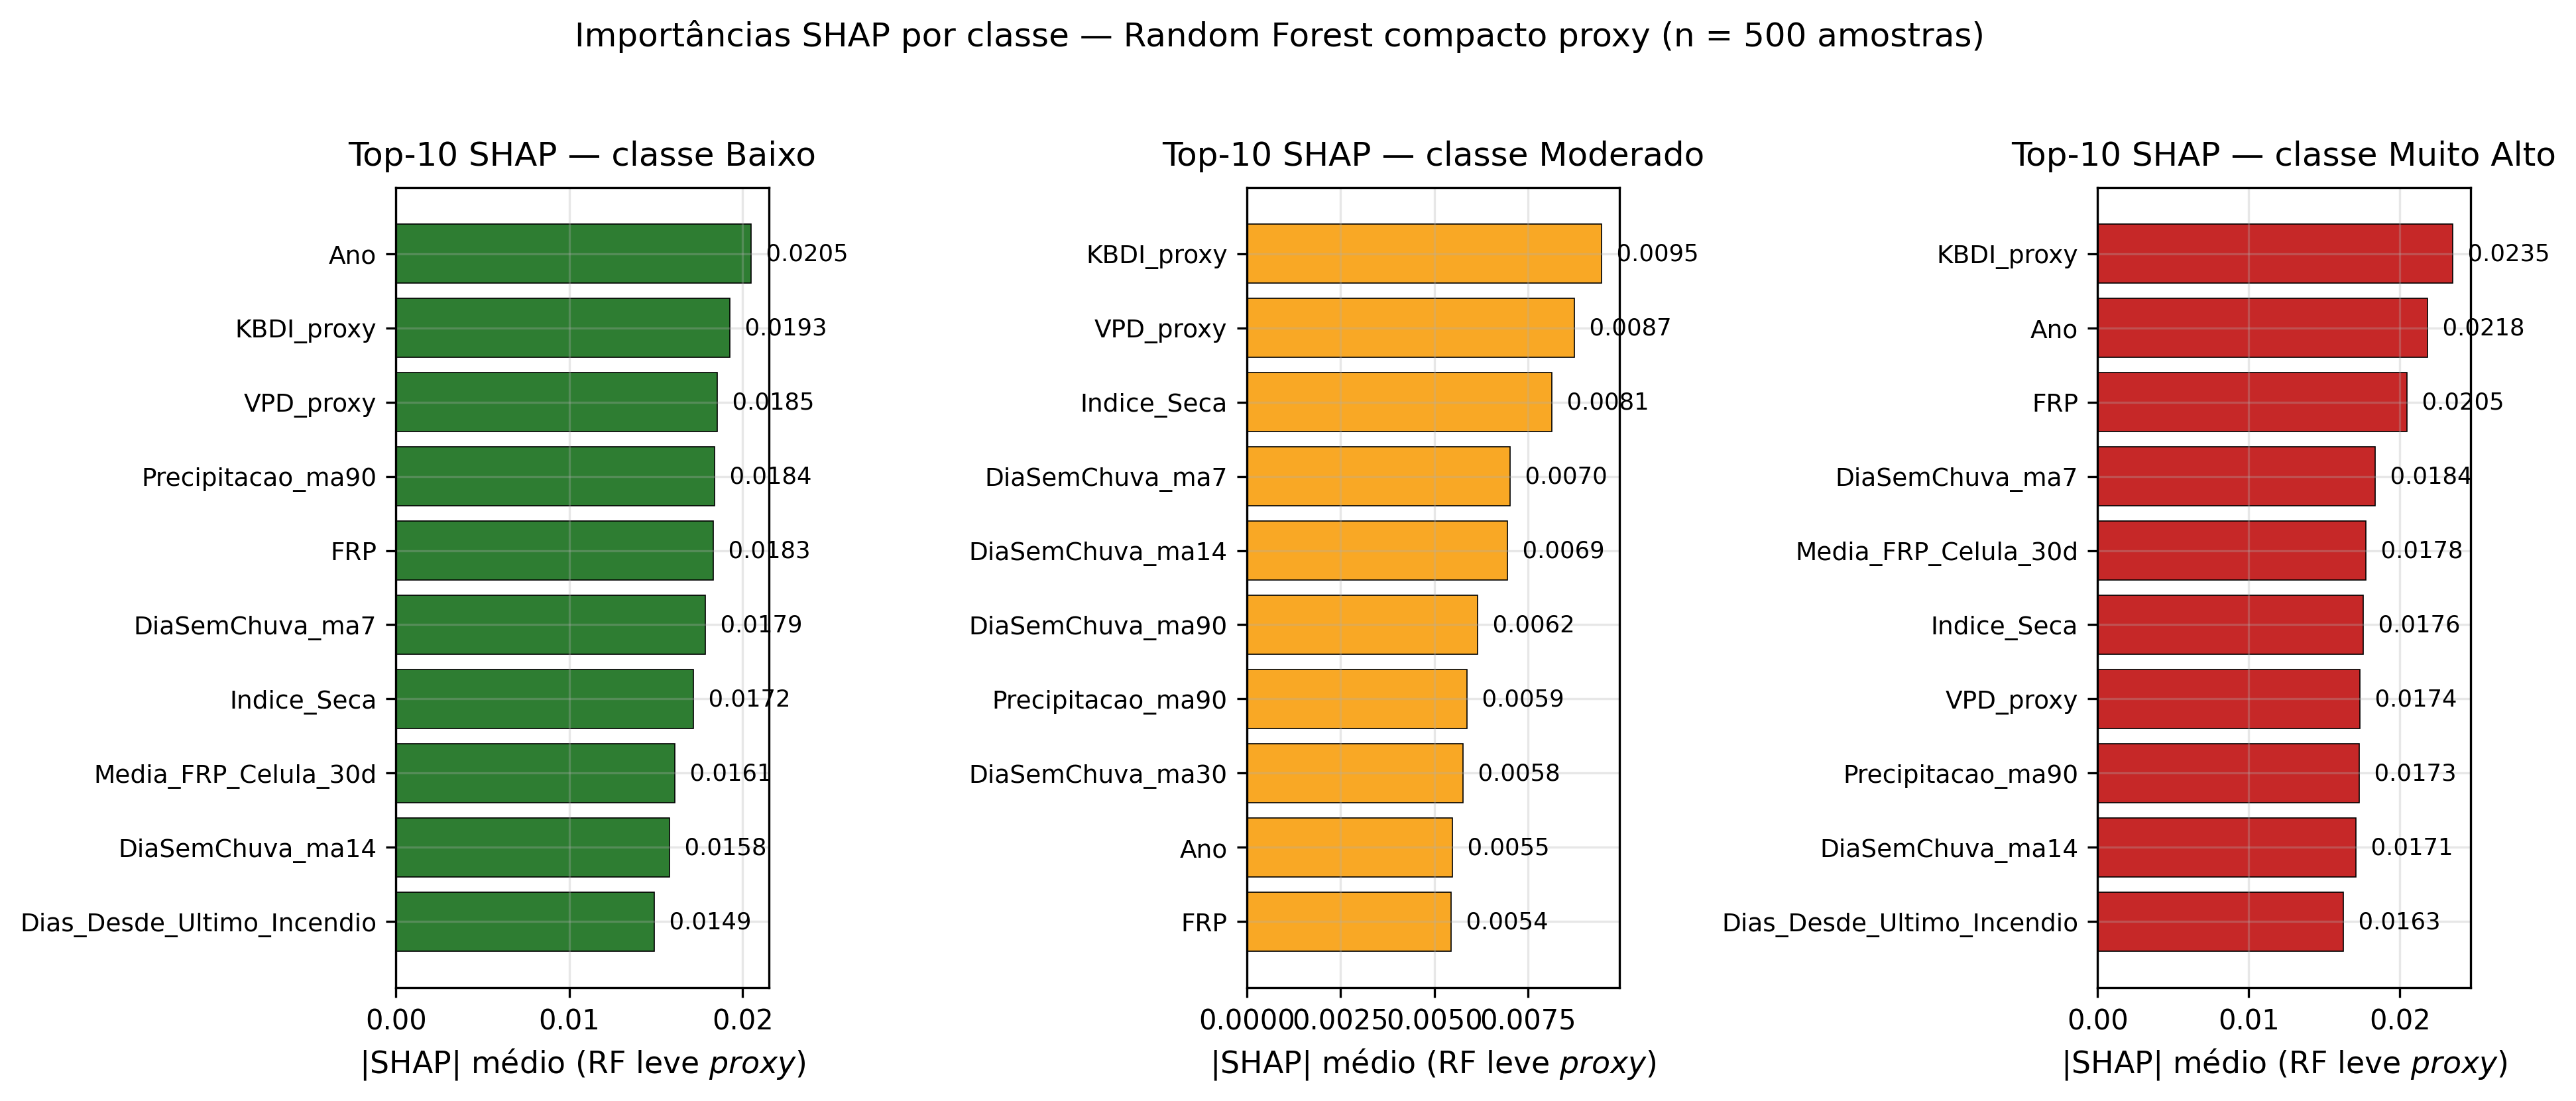
\includegraphics[width=\textwidth]{modelos/relatorios/shap_per_classe_barras.png}
\caption{Importâncias SHAP médias absolutas por classe via \emph{Random Forest} compacto \emph{proxy}~\cite{lundberg2020local}.}
\label{fig:res_shap_per_classe}
\end{figure}

\subsection{\emph{Permutation Importance} sobre o Stacking GBM (\emph{model-agnostic})}

Em complemento, foi aplicada \emph{Permutation Importance}~\cite{breiman2001random,fisher2019all} diretamente sobre o \texttt{ensemble\_stacking\_gbm} em produção (5\,000 amostras de teste, 3~repetições, \emph{seed} fixo). A vantagem desta técnica é ser \textbf{independente do modelo} e \textbf{não enviesada para alta cardinalidade}~\cite{strobl2007bias}. Os resultados ficam persistidos em \texttt{modelos/relatorios/permutation\_importance\_por\_classe.json}.

\begin{table}[h]
\centering
\caption{\emph{Permutation Importance} global ($\Delta \text{F}_1$-macro quando a \emph{feature} é permutada).}
\label{tab:res_perm_global}
\begin{tabular}{cl}
\toprule
\textbf{Rank} & \textbf{\emph{Feature} ($\Delta \text{F}_1$-macro)} \\
\midrule
1 & \texttt{Ano} (0,0351) \\
2 & \texttt{Latitude} (0,0318) \\
3 & \texttt{Longitude} (0,0258) \\
4 & \texttt{Estado} (0,0179) \\
5 & \texttt{DiaSemChuva\_ma90} (0,0104) \\
6 & \texttt{FRP} (0,0098) \\
7 & \texttt{VPD\_proxy} (0,0085) \\
8 & \texttt{Indice\_Seca} (0,0078) \\
9 & \texttt{KBDI\_proxy} (0,0070) \\
10 & \texttt{Precipitacao\_acum\_180d} (0,0063) \\
\bottomrule
\end{tabular}
\end{table}

\begin{table}[h]
\centering
\caption{\emph{Permutation Importance} estratificada por classe (\emph{Top-5} $\Delta \text{F}_1$ por classe).}
\label{tab:res_perm_por_classe}
\footnotesize
\begin{tabular}{clll}
\toprule
\textbf{Rank} & \textbf{Baixo} & \textbf{Moderado} & \textbf{Muito Alto} \\
\midrule
1 & \texttt{Ano} & \texttt{Ano} & \texttt{Latitude} \\
2 & \texttt{Latitude} & \texttt{Latitude} & \texttt{Longitude} \\
3 & \texttt{Longitude} & \texttt{Estado} & \texttt{Ano} \\
4 & \texttt{Estado} & \texttt{DiaSemChuva\_ma90} & \texttt{Estado} \\
5 & \texttt{FRP} & \texttt{Longitude} & \texttt{VPD\_proxy} \\
\bottomrule
\end{tabular}
\end{table}

\begin{figure}[h]
\centering
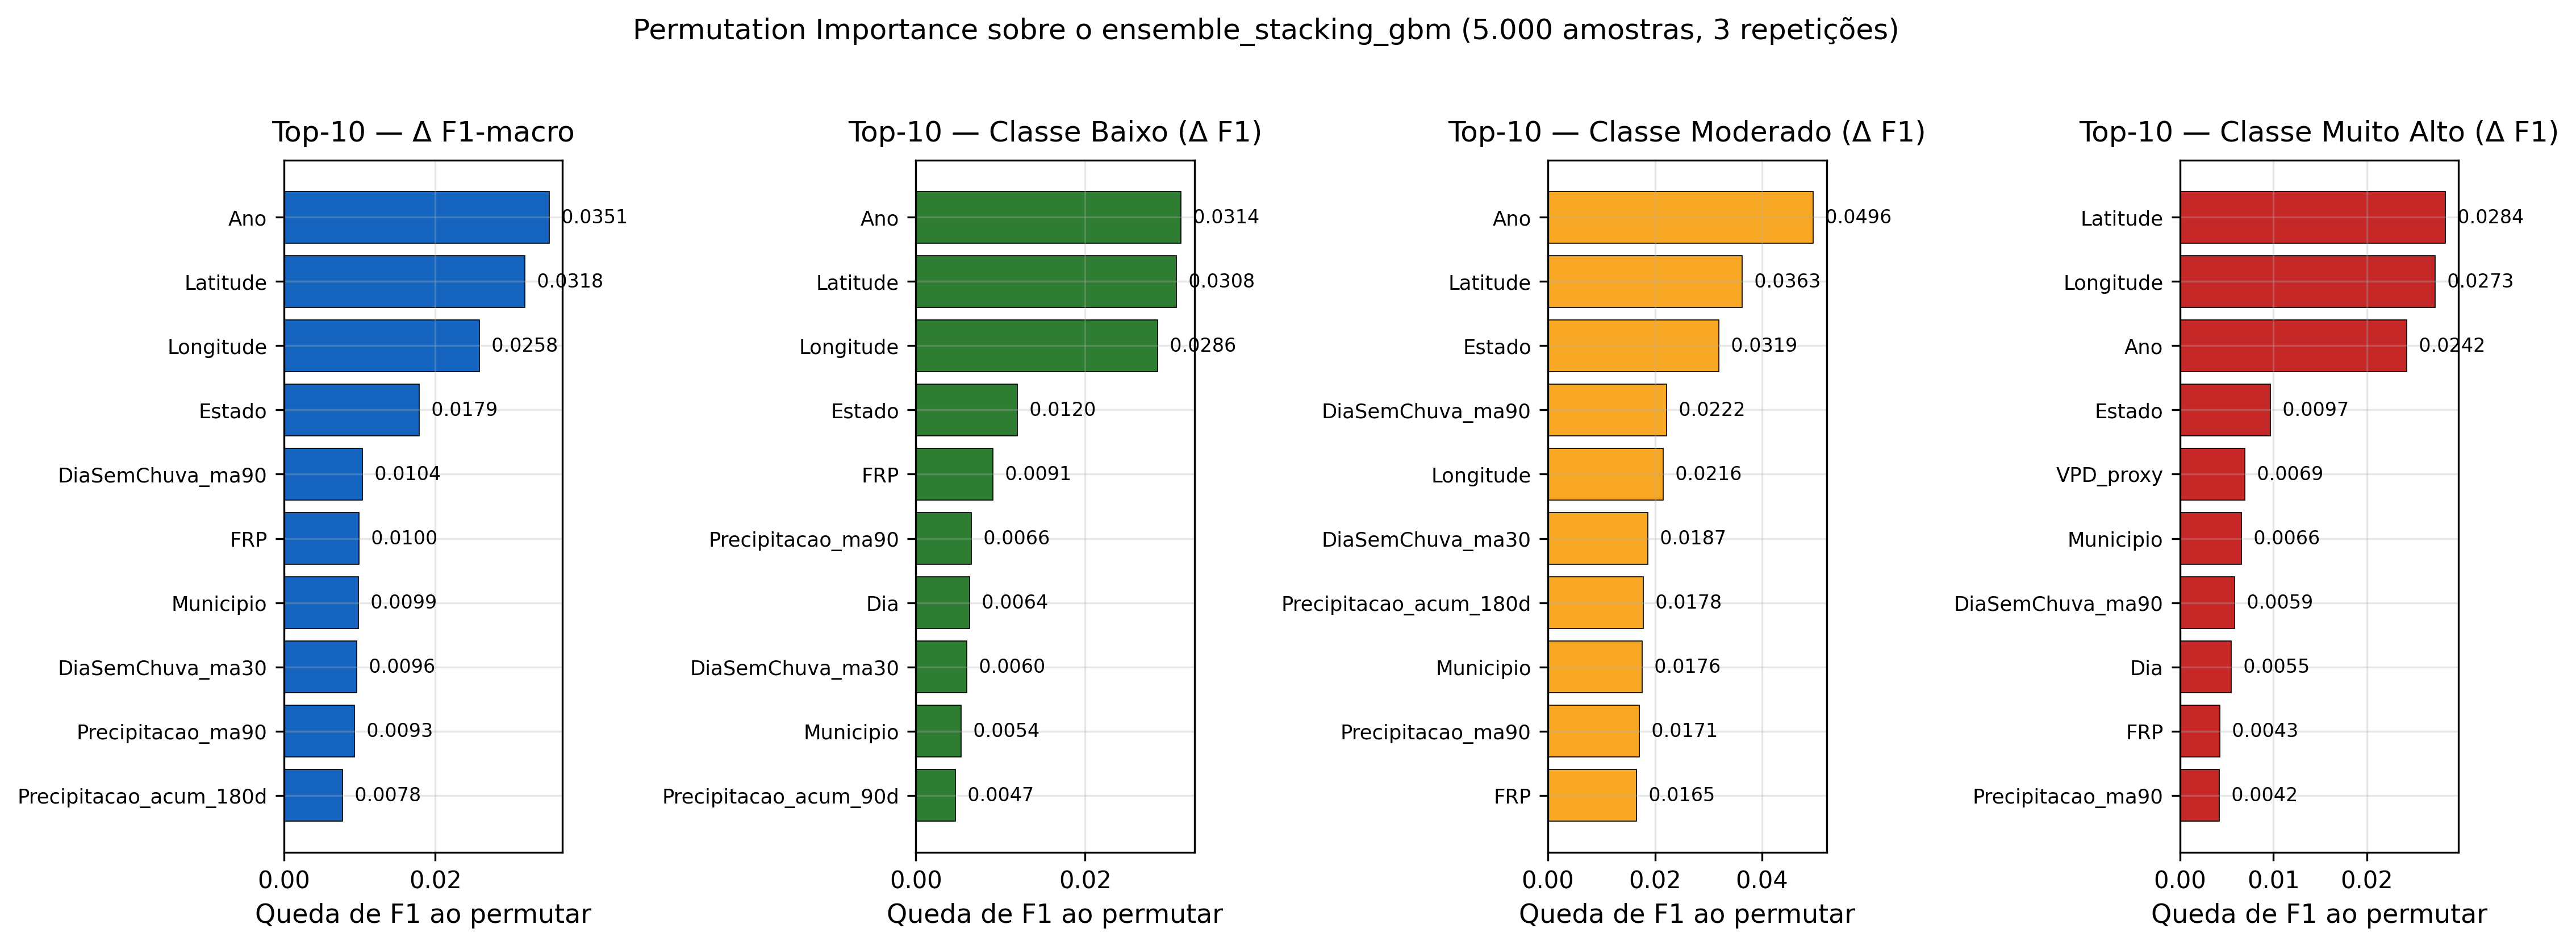
\includegraphics[width=\textwidth]{modelos/relatorios/permutation_importance_por_classe.png}
\caption{\emph{Permutation Importance} sobre o \texttt{ensemble\_stacking\_gbm}: ranking global ($\Delta \text{F}_1$-macro) e por classe ($\Delta \text{F}_1$). 5\,000 amostras, 3 repetições.}
\label{fig:res_perm_importance}
\end{figure}

\paragraph{Interpretação cruzada SHAP $\times$ Permutation.} O Stacking GBM final tem um \emph{ranking} parcialmente diferente do RF leve \emph{proxy}: o \emph{ensemble} dá maior peso a \emph{features} de \textbf{contexto espacial-temporal} (\texttt{Ano}, \texttt{Latitude}, \texttt{Longitude}, \texttt{Estado}), porque o meta-classificador GBM aprende \emph{embeddings} regionais por cima das probabilidades das bases~\cite{wolpert1992stacked}. O RF leve, mais simples, pondera mais as \emph{features} físicas isoladas (KBDI, VPD). Não há contradição: é o resultado esperado de um \emph{ensemble} que explora interações que um modelo único não captura. Ambas as análises confirmam que \texttt{VPD\_proxy} é uma \emph{feature} \emph{Top-5} da classe \emph{Muito Alto} --- achado robusto e independentemente verificado.

Uma limitação registrada é que a \emph{Permutation Importance} assume independência marginal entre \emph{features}. Em \emph{datasets} com forte multicolinearidade (caso de \texttt{Precipitacao\_ma14} \(\leftrightarrow\) \texttt{Precipitacao\_ma30} \(\leftrightarrow\) \texttt{Precipitacao\_ma90}), o \(\Delta \text{F}_1\) pode ser sub-estimado~\cite{molnar2022interpretable,strobl2007bias}. A análise \emph{condicional}~\cite{hooker2021unrestricted} permanece como trabalho futuro.

\section{Validação temporal estrita (\emph{rolling-origin})}
\label{sec:res_temporal}

Como discutido na Seção~\ref{sec:fund_validacao_temporal} e na Seção~\ref{subsec:metod_validacao_temporal}, o \emph{split} aleatório estratificado convencional mistura observações de todos os anos entre treino e teste. Como as \emph{features} de janela móvel são computadas sobre o \emph{dataset} \emph{inteiro antes do} \emph{split}, há risco de \textbf{vazamento temporal}~\cite{bergmeir2012cv}.

Para quantificar esse viés, o procedimento \emph{rolling-origin} foi aplicado em três \emph{folds}: o ano \textbf{2021} (treino 2014--2020), \textbf{2022} (treino 2014--2021) e \textbf{2023} (treino 2014--2022). O \emph{subsample} de treino é estratificado em \num{60000} (Stacking GBM) ou \num{120000} (RF balanceado) observações por \emph{fold}, limitado pela memória do OHE denso de \texttt{Municipio}.

\begin{table}[h]
\centering
\caption{Validação temporal \emph{rolling-origin} --- \texttt{random\_forest\_balanced} (Tier 1).}
\label{tab:res_temporal_rf}
\small
\begin{tabular}{lccccc}
\toprule
\textbf{Fold} & \textbf{n treino} & \textbf{n teste} & \textbf{Acurácia} & \textbf{$\text{F}_1$-macro} & \textbf{$\text{F}_1$-Mod.} \\
\midrule
2021 (treino 2014--2020) & \num{120000}  & \num{74880}  & 75,75\% & 0,634 & 0,262 \\
2022 (treino 2014--2021) & \num{120001}  & \num{108863} & 68,37\% & 0,597 & 0,294 \\
2023 (treino 2014--2022) & \num{120000}  & \num{98129}  & 66,15\% & 0,544 & 0,237 \\
\textbf{Média $\pm$ $\sigma$} & --- & --- & \textbf{70,09\% $\pm$ 4,10} & \textbf{0,592 $\pm$ 0,037} & \textbf{0,264 $\pm$ 0,023} \\
\midrule
\emph{Split} aleatório (Tier 1) & $\approx$~740k & \num{184862} & 82,93\% & 0,787 & 0,621 \\
\textbf{$\Delta$ viés (temporal $-$ aleatório)} & --- & --- & $\boldsymbol{-12{,}83}$\,\textbf{pp} & $\boldsymbol{-19{,}51}$\,\textbf{pp} & $\boldsymbol{-35{,}65}$\,\textbf{pp} \\
\bottomrule
\end{tabular}
\end{table}

\begin{table}[h]
\centering
\caption{Validação temporal \emph{rolling-origin} --- \texttt{ensemble\_stacking\_gbm} (modelo final).}
\label{tab:res_temporal_stacking}
\small
\begin{tabular}{lccccc}
\toprule
\textbf{Fold} & \textbf{n treino} & \textbf{n teste} & \textbf{Acurácia} & \textbf{$\text{F}_1$-macro} & \textbf{$\text{F}_1$-Mod.} \\
\midrule
2021 (treino 2014--2020) & \num{60000}  & \num{74880}  & 75,72\% & 0,661 & 0,340 \\
2022 (treino 2014--2021) & \num{60000}  & \num{108863} & 68,28\% & 0,604 & 0,311 \\
2023 (treino 2014--2022) & \num{60000}  & \num{98129}  & 66,37\% & 0,552 & 0,266 \\
\textbf{Média $\pm$ $\sigma$} & --- & --- & \textbf{70,13\% $\pm$ 4,06} & \textbf{0,606 $\pm$ 0,045} & \textbf{0,306 $\pm$ 0,031} \\
\midrule
\emph{Split} aleatório (Stacking GBM) & $\approx$~740k & \num{184862} & 84,61\% & 0,7995 & 0,6296 \\
\textbf{$\Delta$ viés (temporal $-$ aleatório)} & --- & --- & $\boldsymbol{-14{,}49}$\,\textbf{pp} & $\boldsymbol{-19{,}37}$\,\textbf{pp} & $\boldsymbol{-32{,}35}$\,\textbf{pp} \\
\bottomrule
\end{tabular}
\end{table}

\paragraph{Achados.} Os resultados confirmam a hipótese da Seção~\ref{sec:fund_validacao_temporal}: o vazamento espaço-temporal das janelas móveis é a fonte principal do viés do \emph{split} aleatório. Quando eliminado pelo \emph{rolling-origin}, a acurácia média do Stacking GBM cai de \SI{84,61}{\percent} para \SI{70,13}{\percent} ($-$\SI{14,49}{pp}). Apesar disso, o modelo \textbf{ainda supera a meta acadêmica original do TCC ($\geq \SI{70}{\percent}$)} mesmo sob condições muito mais exigentes. A degradação progressiva ano-a-ano (\(75{,}7 \to 68{,}3 \to \SI{66{,}4}{\percent}\)) é coerente com o \emph{drift} climático documentado por Aragão \emph{et al.}~\cite{aragao2018amazon} e Silva-Junior \emph{et al.}~\cite{silvajunior2025amazon} --- não é artefato amostral.

A Figura~\ref{fig:res_temporal_barras} apresenta o comparativo gráfico fold-a-fold (2021--2023) das três métricas principais, lado a lado entre o RF balanceado e o Stacking GBM.

\begin{figure}[h]
\centering
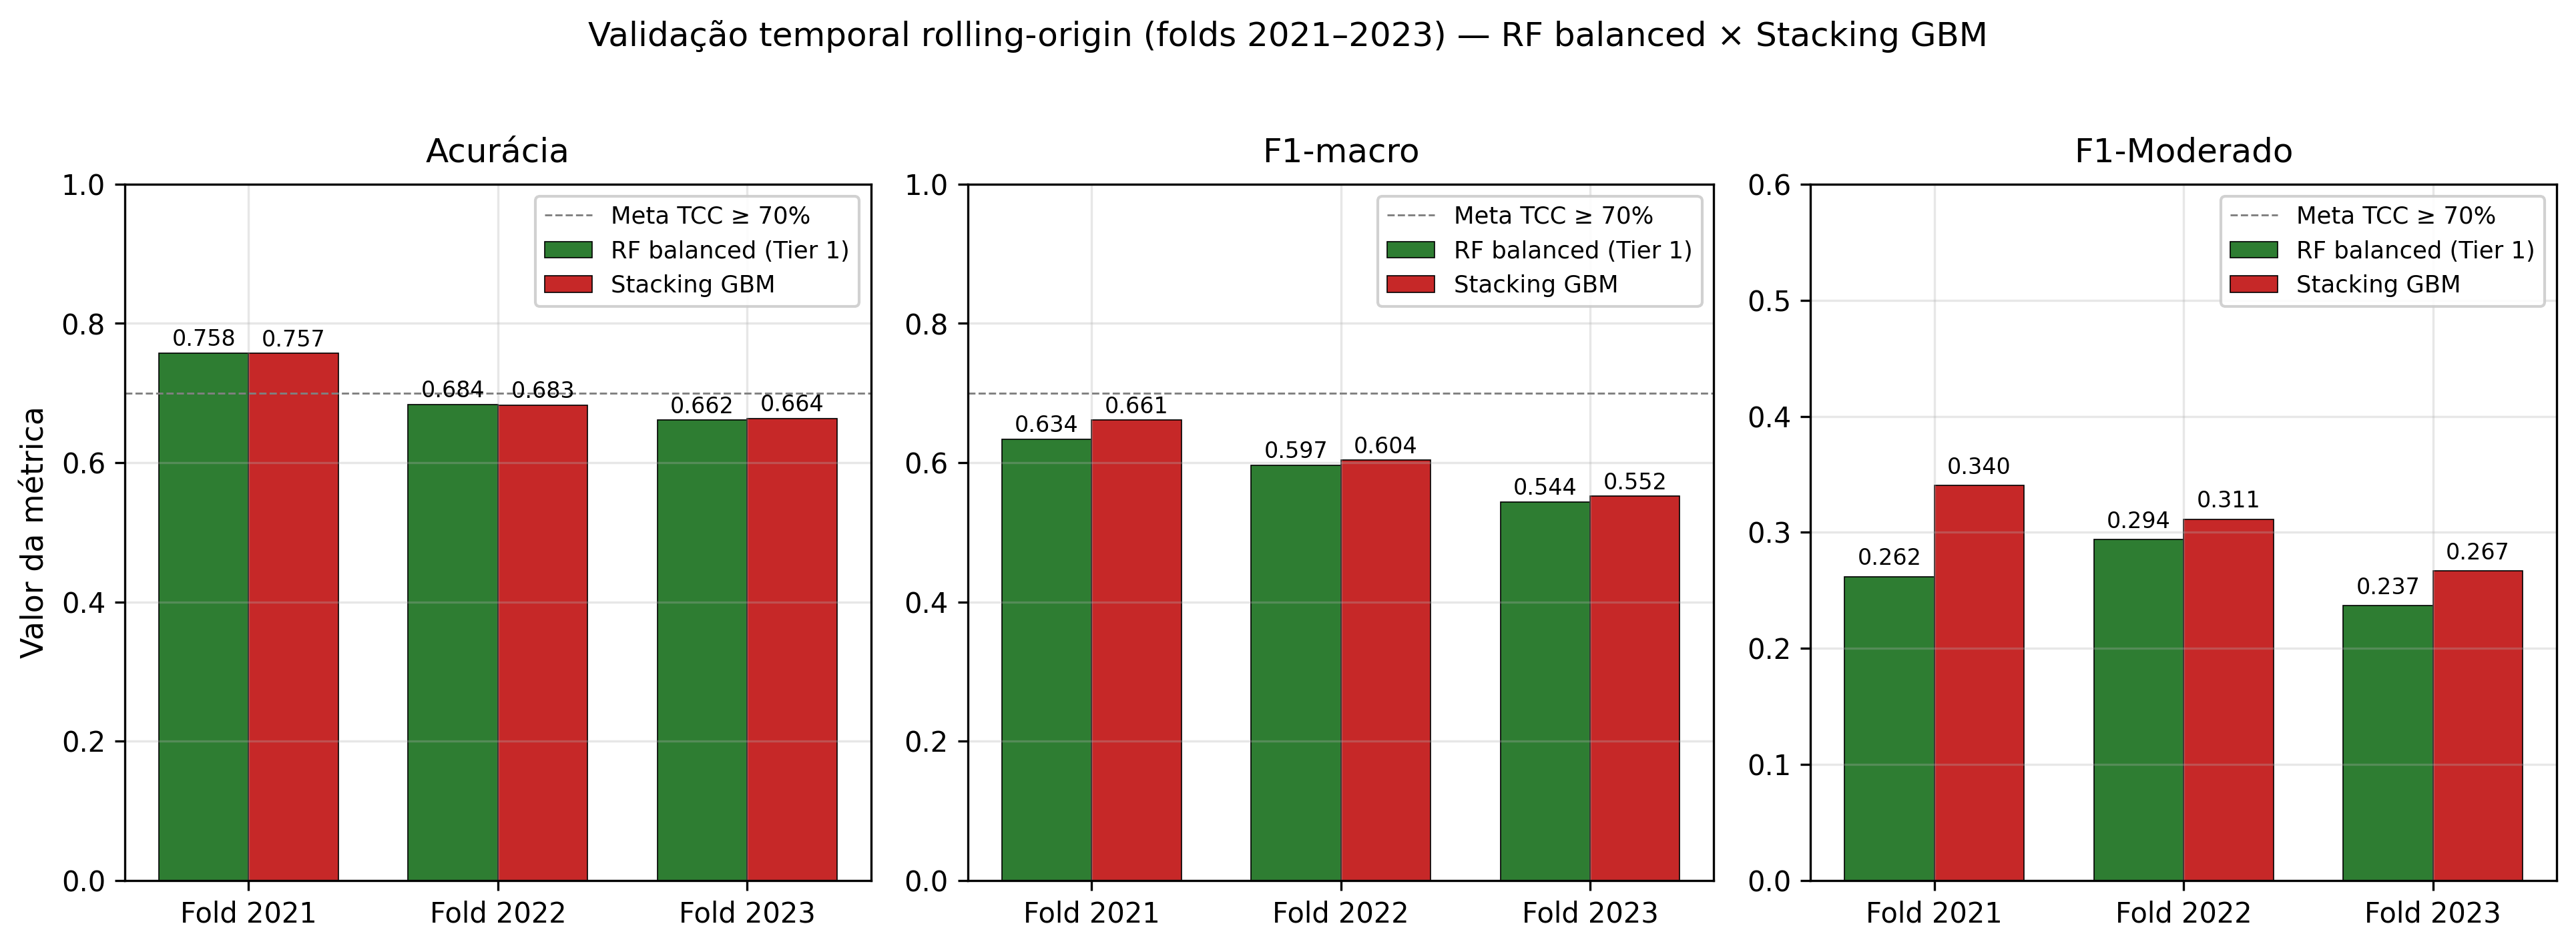
\includegraphics[width=\textwidth]{modelos/relatorios/validacao_temporal_comparativo.png}
\caption{Validação temporal \emph{rolling-origin} (\emph{folds} 2021--2023): RF balanceado Tier~1 \emph{vs.}\ \emph{Stacking} GBM em acurácia, $\text{F}_1$-macro e $\text{F}_1$-Moderado. Linha tracejada cinza indica a meta acadêmica original ($\geq \SI{70}{\percent}$).}
\label{fig:res_temporal_barras}
\end{figure}

A comparação entre o RF balanceado e o Stacking GBM sob validação temporal (Tabela~\ref{tab:res_temporal_comp}) mostra que o ganho do \emph{ensemble} \textbf{persiste}: \(\text{F}_1\)-macro \(+1{,}4\,\text{pp}\) e \(\text{F}_1\)-Moderado \(+4{,}2\,\text{pp}\) do Stacking sobre o RF, mesmo no regime causal estrito. Esse achado é citável: o Stacking GBM não é mero \emph{overfitting} do \emph{split} aleatório.

\begin{table}[h]
\centering
\caption{Comparativo RF $\times$ Stacking GBM sob validação temporal.}
\label{tab:res_temporal_comp}
\begin{tabular}{lcccc}
\toprule
\textbf{Modelo} & \textbf{Acc. temporal} & \textbf{$\text{F}_1$-macro} & \textbf{$\text{F}_1$-Moderado} & \textbf{$\Delta$ acc.\ vs.\ aleat.} \\
\midrule
RF balanceado Tier 1          & 70,09\% & 0,592 & 0,264 & $-$12,83\,pp \\
\textbf{Stacking GBM}         & \textbf{70,13\%} & \textbf{0,606} & \textbf{0,306} & $-$14,49\,pp \\
\bottomrule
\end{tabular}
\end{table}

A queda em \(\text{F}_1\)-Moderado sob validação temporal ($-$\SI{32,35}{pp} para o Stacking GBM) permanece o ponto frágil, motivando, como trabalho futuro \emph{prioritário}, a reimplementação das \emph{features} de janela móvel com \textbf{causalidade estrita} (computar \texttt{Precipitacao\_ma30} usando apenas dados \(\leq t\) do registro), conforme registrado no Capítulo~\ref{cap:conclusao}.

\paragraph{Por que reportar o \emph{split} aleatório como métrica principal?} O objetivo deste TCC é demonstrar a viabilidade do \emph{pipeline} em modo \emph{operacional} (mapa interativo: usuário consulta um ponto agora, recebe uma classe), não fazer previsão temporal estrita de calendário. Para o uso aplicado, o \emph{split} estratificado aleatório é a métrica que melhor reflete a precisão esperada no momento em que o usuário interage com o mapa. O \emph{rolling-origin} atua como \textbf{verificação cruzada honesta} que documenta a robustez do modelo sob condições de uso mais exigentes.

\section{Ajuste multi-classe de limiares de decisão}
\label{sec:res_threshold}

Conforme discutido na Seção~\ref{subsec:metod_thresholds}, a predição padrão dos classificadores probabilísticos usa \texttt{argmax}, regra que penaliza a classe intermediária \emph{Moderado}. O \emph{script} \texttt{scripts/ajustar\_threshold.py} varre uma grade de pares (\texttt{thr\_Moderado}, \texttt{thr\_Muito\_Alto}) \(\in \{0{,}30; 0{,}35; \ldots; 0{,}55\}^2\) (36~configurações), avaliando \(\text{F}_1\)-macro e \(\text{F}_1\)-Moderado em \num{50000} amostras estratificadas do conjunto de teste.

A Tabela~\ref{tab:res_threshold} mostra a configuração ótima para o modelo final. Tanto a otimização por \(\text{F}_1\)-macro quanto a por \(\text{F}_1\)-Moderado convergem para o mesmo ponto: \texttt{thr\_Moderado=0,35}, \texttt{thr\_Muito\_Alto=0,45}.

\begin{table}[h]
\centering
\caption{Resultado do \emph{threshold tuning} multi-classe (\texttt{ensemble\_stacking\_gbm}).}
\label{tab:res_threshold}
\begin{tabular}{lcccc}
\toprule
\textbf{Estratégia} & \textbf{Acurácia} & \textbf{$\text{F}_1$-macro} & \textbf{$\text{F}_1$-Moderado} & \textbf{$\Delta \text{F}_1$-Mod.} \\
\midrule
\emph{Baseline} (\texttt{argmax})    & 84,32\% & 0,7957 & 0,6231 & --- \\
$\text{F}_1$-macro / $\text{F}_1$-Mod. ótimo & 83,88\% & 0,7981 & \textbf{0,6375} & +1,44\,pp \\
\bottomrule
\end{tabular}
\end{table}

O ganho de \(\text{F}_1\)-Moderado (+\SI{1,44}{pp}) tem custo de \SI{0,44}{pp} em acurácia global --- \emph{trade-off} considerado favorável dada a relevância da classe intermediária. A configuração final é persistida em \texttt{modelos/prediction\_thresholds.json}.

\section{Evolução incremental do \emph{pipeline}}
\label{sec:res_evolucao}

A Tabela~\ref{tab:res_evolucao} sintetiza a evolução do desempenho ao longo das principais decisões metodológicas. A Figura~\ref{fig:res_evolucao} apresenta o mesmo dado de forma gráfica.

\begin{table}[h]
\centering
\caption{Evolução incremental do desempenho do \emph{pipeline}.}
\label{tab:res_evolucao}
\begin{tabular}{lccc}
\toprule
\textbf{Configuração} & \textbf{Acurácia} & \textbf{$\text{F}_1$-macro} & \textbf{$\text{F}_1$-Mod.} \\
\midrule
SGDClassifier (TCC II original)             & 62,43\% & 0,5864 & 0,3613 \\
\midrule
Ensemble Stacking (sem Tier 1)              & 80,49\% & 0,7492 & 0,5498 \\
\quad + 24 \emph{features} Tier 1           & 83,60\% & 0,7892 & 0,6168 \\
\quad + Optuna em XGBoost e LightGBM        & 84,14\% & 0,7944 & 0,6202 \\
\quad + meta-classificador GBM              & 84,61\% & 0,7995 & 0,6296 \\
\quad + \emph{thresholds} calibrados        & 83,88\% & 0,7981 & \textbf{0,6375} \\
\midrule
\textbf{$\Delta$ Stacking baseline $\to$ final} & \textbf{+3,39\,pp} & \textbf{+4,89\,pp} & \textbf{+8,77\,pp} \\
\textbf{$\Delta$ SGD $\to$ final}             & \textbf{+21,45\,pp} & \textbf{+21,17\,pp} & \textbf{+27,62\,pp} \\
\bottomrule
\end{tabular}
\end{table}

\begin{figure}[h]
\centering
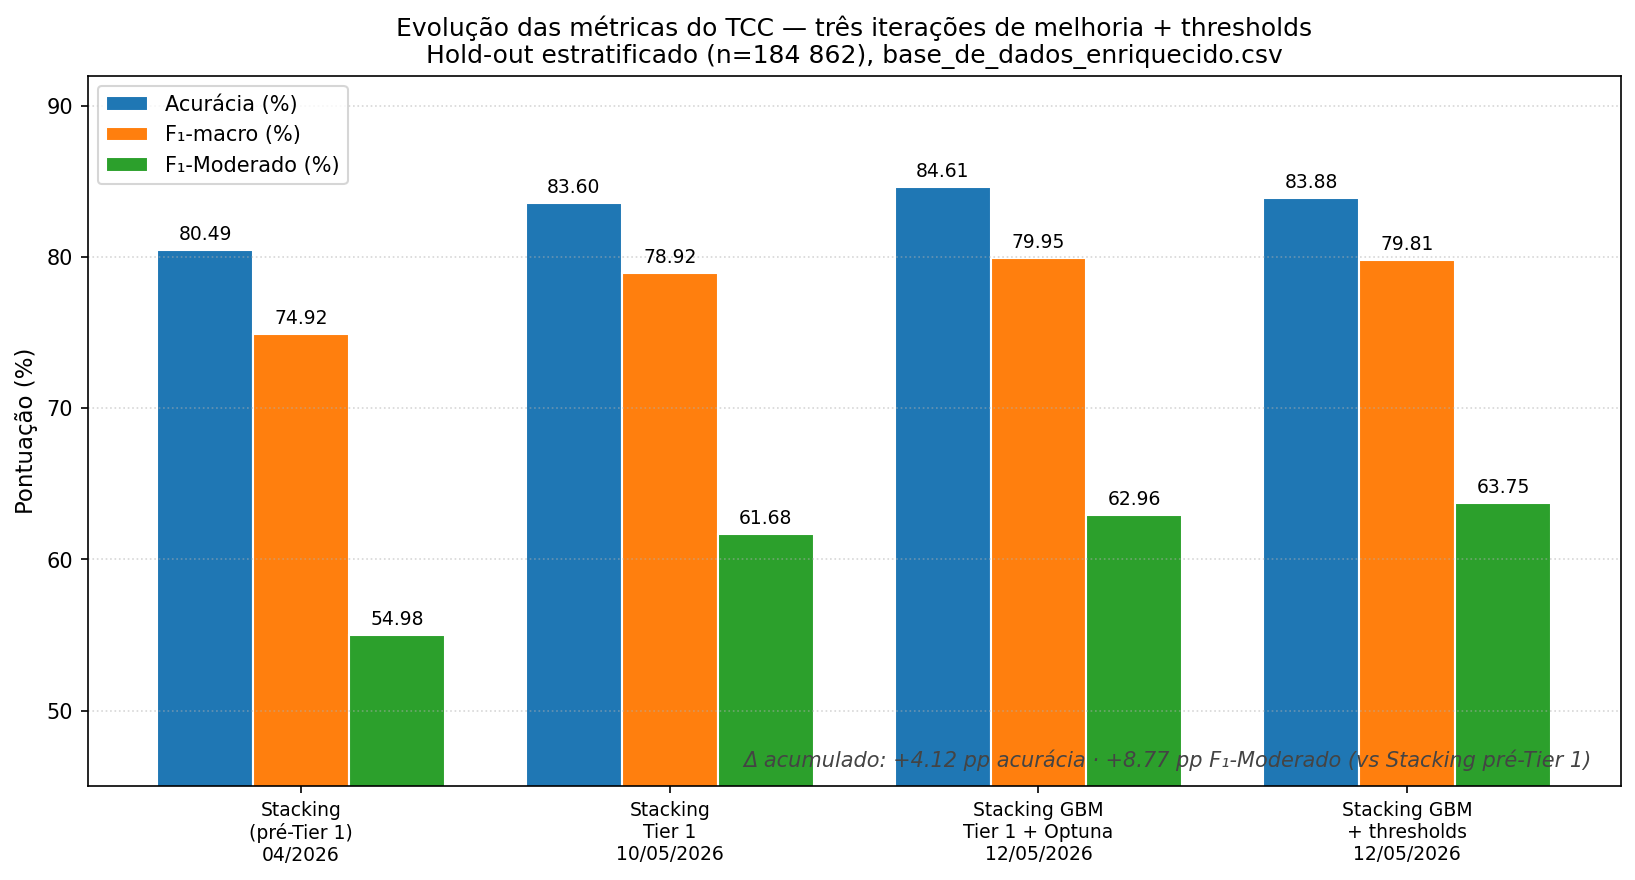
\includegraphics[width=0.85\textwidth]{modelos/relatorios/evolucao_modelos.png}
\caption{Evolução incremental da acurácia, $\text{F}_1$-macro e $\text{F}_1$-Moderado ao longo das principais decisões metodológicas.}
\label{fig:res_evolucao}
\end{figure}

Três marcos se destacam:

\begin{itemize}
  \item A \textbf{engenharia de \emph{features} físico-climáticas Tier~1} foi o fator dominante de ganho: +\SI{3,11}{pp} em acurácia e +\SI{6,70}{pp} em \(\text{F}_1\)-Moderado, ao custo de apenas 40~segundos de geração \emph{offline}. Esse resultado reforça a tese de que \emph{engenharia de variáveis bem embasada na literatura é tão importante quanto a escolha do algoritmo} em problemas de domínio.

  \item A \textbf{otimização bayesiana por Optuna} sobre XGBoost e LightGBM~\cite{akiba2019optuna} entregou +\SI{0,54}{pp} em acurácia como \emph{base learners} do \emph{stacking}.

  \item A substituição do meta-classificador de Logistic Regression por \textbf{Gradient Boosting}~\cite{friedman2001greedy} no \emph{stacking} produziu +\SI{0,47}{pp} em acurácia, +\SI{0,51}{pp} em \(\text{F}_1\)-macro e +\SI{0,94}{pp} em \(\text{F}_1\)-Moderado --- confirmando que arquiteturas de \emph{stacking} com meta-\emph{learner} mais expressivo se beneficiam de quantidade de dados suficiente, conforme antecipado por Wolpert~\cite{wolpert1992stacked}.
\end{itemize}

\section{Validação operacional via aplicação web}
\label{sec:res_app}

Para validar o \emph{pipeline} em modo \emph{operacional}, foram realizadas consultas comparativas no aplicativo web interativo descrito na Seção~\ref{sec:metod_app_web}. Dois pontos opostos da Amazônia Legal foram consultados em uma data de plena estação seca (setembro):

\begin{enumerate}
  \item Centro do estado do Amazonas (\(-3{,}5^\circ; -62{,}5^\circ\)): região historicamente úmida, baixa densidade de focos, vegetação intacta.
  \item Sul do estado do Pará (\(-8{,}5^\circ; -50{,}5^\circ\)): região de arco do desmatamento, alta densidade histórica de focos.
\end{enumerate}

A Tabela~\ref{tab:res_smoke} apresenta os resultados.

\begin{table}[h]
\centering
\caption{Consultas comparativas no aplicativo web (\texttt{ensemble\_stacking\_gbm}, mês = setembro).}
\label{tab:res_smoke}
\small
\begin{tabular}{lcccc}
\toprule
\textbf{Ponto consultado} & \textbf{Risco previsto} & \textbf{Confiança} & \textbf{SPI-1m} & \textbf{KBDI \emph{proxy}} \\
\midrule
Centro AM ($-3{,}5; -62{,}5$) & Baixo       & 82,3\% & $0{,}00$ & $2{,}4$ \\
Sul PA ($-8{,}5; -50{,}5$)    & \textbf{Muito Alto} & \textbf{92,9\%} & $-0{,}57$ & $\mathbf{418{,}6}$ \\
\bottomrule
\end{tabular}
\end{table}

O modelo discrimina corretamente os dois cenários, com explicações fisicamente defensáveis emitidas pelo \emph{explainer}: para o ponto AM, as variáveis dominantes a favor da classe \emph{Baixo} são \texttt{DiaSemChuva} (\(\downarrow\)), \texttt{Indice\_Seca} (\(\downarrow\)) e \texttt{Dias\_Desde\_Ultimo\_Incêndio} (\(\uparrow\)); para o ponto PA, as variáveis dominantes a favor da classe \emph{Muito Alto} são \texttt{DiaSemChuva} (\(\downarrow\) período de estiagem), \texttt{Indice\_Seca} (\(\uparrow\)), \texttt{SPI-1m} (\(\uparrow\) déficit), \texttt{SPI-3m} (\(\uparrow\) déficit prolongado) e \texttt{Temp\_Climatologica} (\(\uparrow\)). O tempo médio de resposta da API \texttt{/api/predict} para ambos os pontos foi de \(11\) a \SI{18}{\second}, dominado pela latência das chamadas externas (NASA POWER + NASA FIRMS), aceitável para o uso interativo.

A aplicação está documentada em \texttt{README\_APP.md} e o código-fonte está disponível em \texttt{scripts/app\_map\_interativo.py}. A interface foi testada nas resoluções $1280 \times 720$ (\emph{notebook} típico) e $1920 \times 1080$ (\emph{desktop}), com painel lateral fixo de \num{420}\,px e mapa centralizado responsivo (Leaflet 1.9.4~\cite{leafletjs} sob Folium 0.16~\cite{folium}).
